\documentclass[a4paper, fontsize = 8pt, landscape]{scrartcl}
\usepackage{../../../misc_files/LateX/layout_and_colours}
\makeatletter
\def\input@path{{content/old/}{content/examples/}}
\makeatother
\graphicspath{{content/}{content/summary/}{content/examples/}}

\title{Software Entwicklung 1}
\author{Jil Zerndt, Lucien Perret}
\date{January 2025}

\createtitlepagestyle
\createmainpagestyle
\begin{document}
\begin{multicols}{3}
	\thispagestyle{TitlePageStyle}
	\maketitle
	\pagebreak
    \section{Einführung und Überblick}

\begin{definition}{Software Engineering}
\begin{itemize}
    \item Disziplinen: Anforderungen, Architektur, Implementierung, Test und Wartung.
    \item Ziel: Strukturierte Prozesse für Qualität, Risiko- und Fehlerminimierung.
\end{itemize}
\end{definition}

\begin{definition}{Modellierung in der Softwareentwicklung}
\begin{itemize}
    \item Modelle als Abstraktionen: Anforderungen, Architekturen, Testfälle.
    \item Einsatz von UML: Skizzen, detaillierte Blueprints, vollständige Spezifikationen.
    \end{itemize}
\end{definition}

\begin{concept}{Wrap-up}
\begin{itemize}
    \item Solide Analyse- und Entwurfskompetenzen sind essenziell.
    \item Iterativ-inkrementelle Modelle fördern agile Entwicklung.
\end{itemize}
\end{concept}

\subsection{Softwareentwicklungsprozesse}

\begin{concept}{Klassifizierung Software-Entwicklungs-Probleme}\\
  Wir betrachten Wasserfall, iterativ-inkrementelle und agile Softwareentwicklungsprozesse.\\
  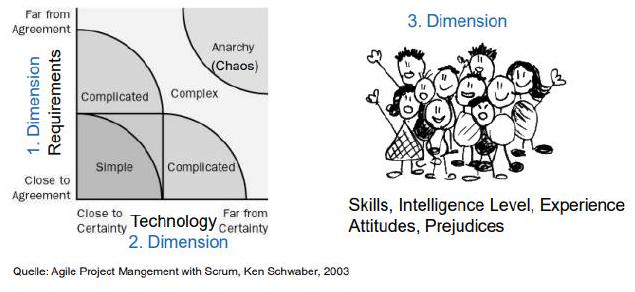
\includegraphics[width=\linewidth]{images/2024_12_29_0d1d7b5551ea1b4b41bdg-01}
\end{concept}


\begin{theorem}{Prozesse im Softwareengineering Kernprozesse}
\begin{itemize}
  \item Anforderungserhebung
  \item Systemdesign/technische Konzeption
  \item Implementierung
  \item Softwaretest
  \item Softwareeinführung
  \item Wartung/Pflege
\end{itemize}
\end{theorem}

\begin{corollary}{Unterstützungsprozesse}
\begin{itemize}
  \item Projektmanagement
  \item Qualitätsmanagement
  \item Risikomanagement
\end{itemize}
\end{corollary}

\begin{definition}{Begriffe}
  \begin{itemize}
    \item Warum wird modelliert: Um Analyse- und Designentwürfe zu diskutieren, abstimmen und zu dokumentieren bzw. zu kommunizieren.
    \item Modell: Ein Modell ist ein konkretes oder gedankliches Abbild eines vorhanden Gebildes oder Vorbild für ein zu schaffendes Gebilde (hier Softwareprodukt).
    \item Original: Das Original ist das abgebildete oder zu schaffende Gebilde.
    \item Modellierung: Modellierung gehört zum Fundament des Software Engineerings
  \end{itemize}
\end{definition}

\begin{concept}{Modelle in der Softwareentwicklung}
\begin{itemize}
  \item Software ist vielfach (immer?) selbst ein Modell
  \item Anforderungen sind Modelle der Problemstellung
  \item Architekturen und Entwürfe sind Modelle der Lösung
  \item Testfälle sind Modelle des korrekten Funktionierens des Codes usw.
\end{itemize}
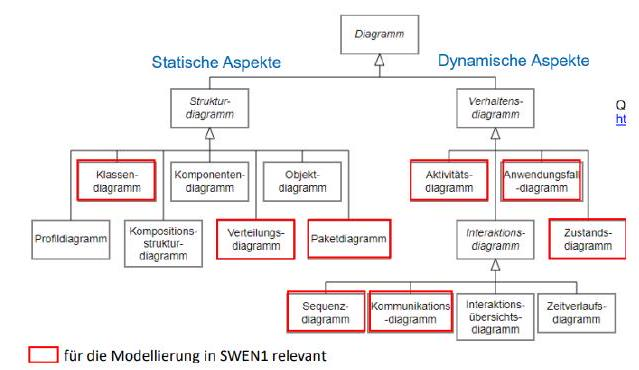
\includegraphics[width=\linewidth]{images/2024_12_29_0d1d7b5551ea1b4b41bdg-01(1)}
\end{concept}

\begin{definition}{Code and Fix}\\
Vorgehen, bei dem Codierung oder Korrektur im Wechsel mit Ad-hoc-Tests die einzigen bewussten ausgeführten Tätigkeiten der Software-Entwicklung sind: Schnell, Agil, Einfach am Anfang, Schlecht Planbar, Schlecht Wartbar, Änderungen s. Aufwändig
\end{definition}

\begin{definition}{Wasserfallmodell}\\
Die Software-Entwicklung wird als Folge von Aktivitäten/Phasen betrachtet, die durch Teilergebnisse (Dokumente) gekoppelt sind. Die Reihenfolge der Ak-\\
tivitäten ist fest definiert. : gut planbar, klare Aufteilung in Phasen, Schlechtes Risikomanagment, nie alle Anforderungen zu Anfang bekannt
\end{definition}

\begin{definition}{Iterativ-inkrementelle Modelle}\\
Software wird in mehreren geplanten und kontrolliert durchgeführten Iterationen schrittweise (inkrementell) entwickelt: Flexibles Modell, Gutes Risikomanagement, Frühe Einsetzbarkeit, Planung upfront hat Grenzen, Kunde Involviert über ganze Entwicklung\\
Agile Softwareentwicklung Basiert auf interativ-inkrementellen Prozessmodell, Fokussiert auf gut dokumentierten und getesteten Code statt auf ausführlicher Dokumentation
\end{definition}

\begin{concept}{Zweck und den Nutzen von Modellen in der Softwareentwicklung}\\
Modell von Requirements (close to/ far from Agreement) \& Technology (known / unknown)\\
Ein Modell ist ein konkretes oder gedankliches Abbild eines vorhanden Gebildes oder Vorbild für ein zu schaffendes Gebilde (hier Softwareprodukt).
\end{concept}

\begin{definition}{Unified Modelling Language (UML)}\\
UML ist die Standardsprache für die graphische Modellierung von Anforderungen, Analyse und Entwürfen im Software Engineering (objektorientierte Modellierung). (As a sketch, blueprint, programminglanguage)
\end{definition}

\begin{formula}{Incremental Model}\\
  Artefakte in einem iterativ-inkrementellen Prozess illustrieren und einordnen\\
\begin{center}
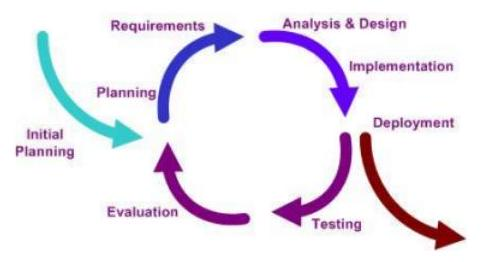
\includegraphics[width=0.8\linewidth]{images/2024_12_29_0d1d7b5551ea1b4b41bdg-02(1)}
\end{center}
\end{formula}
	\raggedcolumns
	\pagebreak
    \section{Anforderungsanalyse}

\subsubsection{Usability und User Experience}

\begin{concept}{Usability und User Experience}\\
Die drei Säulen der Benutzererfahrung:
\begin{itemize}
    \item \textbf{Usability (Gebrauchstauglichkeit):} Grundlegende Nutzbarkeit des Systems
    \item \textbf{User Experience:} Usability + Desirability (Attraktivität)
    \item \textbf{Customer Experience:} UX + Brand Experience (Markenwahrnehmung)
\end{itemize}
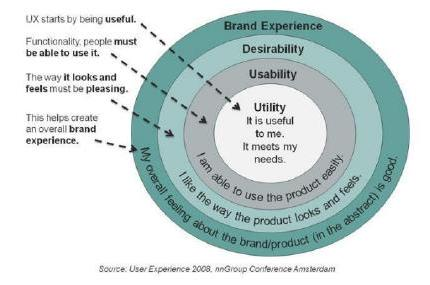
\includegraphics[width=0.9\linewidth]{images/2024_12_29_0d1d7b5551ea1b4b41bdg-02}
\end{concept}

\begin{definition}{Usability-Dimensionen}\\
Die drei Hauptdimensionen der Usability:
\begin{itemize}
    \item \textbf{Effektivität:}
    \begin{itemize}
        \item Vollständige Aufgabenerfüllung
        \item Gewünschte Genauigkeit
    \end{itemize}
    \item \textbf{Effizienz:} Minimaler Aufwand
    \begin{itemize}
        \item Mental
        \item Physisch
        \item Zeitlich
    \end{itemize}
    \item \textbf{Zufriedenheit:}
    \begin{itemize}
        \item Minimum: Keine Verärgerung
        \item Standard: Zufriedenheit
        \item Optimal: Begeisterung
    \end{itemize}
\end{itemize}
\end{definition}

\begin{theorem}{ISO 9241-110: Usability-Anforderungen}\\
Die sieben Grundprinzipien:
\begin{itemize}
    \item Aufgabenangemessenheit
    \item Lernförderlichkeit
    \item Individualisierbarkeit
    \item Erwartungskonformität
    \item Selbstbeschreibungsfähigkeit
    \item Steuerbarkeit
    \item Fehlertoleranz
\end{itemize}
\end{theorem}

\begin{concept}{User-Centered Design (UCD)}\\
Ein iterativer Prozess zur nutzerzentrierten Entwicklung:\\
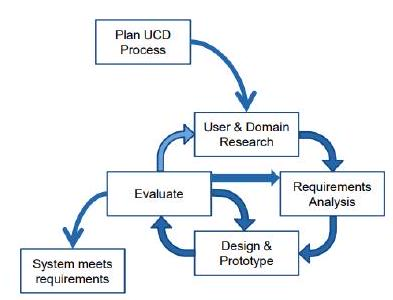
\includegraphics[width=0.6\linewidth]{images/2024_12_29_0d1d7b5551ea1b4b41bdg-03}
\end{concept}
\begin{theorem}{Wichtige Artefakte}
\begin{itemize}
    \item Personas: Repräsentative Nutzerprofile
    \item Usage-Szenarien: Konkrete Anwendungsfälle
    \item Mentales Modell: Nutzerverständnis
    \item Domänenmodell: Fachliches Verständnis
    \item Service Blueprint: Geschäftsprozessmodell
    \item Stakeholder Map: Beteiligte und Betroffene
    \item UI-Artefakte: Skizzen, Wireframes, Designs
\end{itemize}
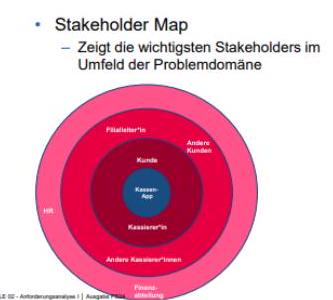
\includegraphics[width=0.5\linewidth]{images/2024_12_29_0d1d7b5551ea1b4b41bdg-04}
\end{theorem}

\subsubsection{Requirements Engineering}

\begin{definition}{Requirements (Anforderungen)}
\begin{itemize}
    \item Leistungsfähigkeiten oder Eigenschaften
    \item Explizit oder implizit
    \item Müssen mit allen Stakeholdern erarbeitet werden
    \item Entwickeln sich während des Projekts
\end{itemize}
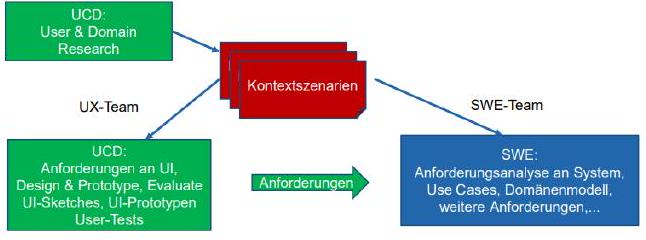
\includegraphics[width=\linewidth]{images/2024_12_29_0d1d7b5551ea1b4b41bdg-04(1)}
\end{definition}

\subsection{Use Cases}

\begin{definition}{Use Case (Anwendungsfall)}\\
Textuelle Beschreibung einer konkreten Interaktion zwischen Akteur und System:
\begin{itemize}
    \item Aus Sicht des Akteurs
    \item Aktiv formuliert
    \item Konkreter Nutzen
    \item Essentieller Stil (Logik statt Implementierung)
\end{itemize}
\end{definition}

\begin{theorem}{Akteure in Use Cases}
\begin{itemize}
    \item \textbf{Primärakteur:} Initiiert den Use Case, erhält Hauptnutzen
    \item \textbf{Unterstützender Akteur:} Hilft bei der Durchführung
    \item \textbf{Offstage-Akteur:} Indirekt beteiligter Stakeholder
\end{itemize}
\end{theorem}

\begin{KR}{Use Case Erstellung}\\
Schritte zur Erstellung eines vollständigen Use Cases:
\begin{enumerate}
    \item \textbf{Identifikation:}
    \begin{itemize}
        \item Systemgrenzen definieren
        \item Primärakteure identifizieren
        \item Ziele der Akteure ermitteln
    \end{itemize}
    \item \textbf{Dokumentation:}
    \begin{itemize}
        \item Brief/Casual für erste Analyse
        \item Fully-dressed für wichtige Use Cases
        \item Standardablauf und Erweiterungen
    \end{itemize}
    \item \textbf{Review:}
    \begin{itemize}
        \item Mit Stakeholdern abstimmen
        \item Auf Vollständigkeit prüfen
        \item Konsistenz sicherstellen
    \end{itemize}
\end{enumerate}
\end{KR}

\begin{example2}{Brief Use Case}
\textbf{Verkauf abwickeln}

Kunde kommt mit Waren zur Kasse. Kassier erfasst alle Produkte. System berechnet Gesamtbetrag. Kassier nimmt Zahlung entgegen und gibt ggf. Wechselgeld. System druckt Beleg.
\end{example2}

\begin{example2}{Fully-dressed Use Case}
\textbf{UC: Verkauf abwickeln}
\begin{itemize}
    \item \textbf{Umfang:} Kassensystem
    \item \textbf{Primärakteur:} Kassier
    \item \textbf{Stakeholder:} Kunde (schnelle Abwicklung), Geschäft (korrekte Abrechnung)
    \item \textbf{Vorbedingung:} Kasse ist geöffnet
    \item \textbf{Standardablauf:}
    \begin{enumerate}
        \item Kassier startet neuen Verkauf
        \item System initialisiert neue Transaktion
        \item Kassier erfasst Produkte
        \item System zeigt Zwischensumme
        \item Kassier schliesst Verkauf ab
        \item System zeigt Gesamtbetrag
        \item Kunde bezahlt
        \item System druckt Beleg
    \end{enumerate}
\end{itemize}
\end{example2}

\begin{concept}{Systemsequenzdiagramm (SSD)}\\
Formalisierte Darstellung der System-Interaktionen:
\begin{itemize}
    \item Zeigt Input/Output-Events
    \item Identifiziert Systemoperationen
    \item Basis für API-Design
\end{itemize}
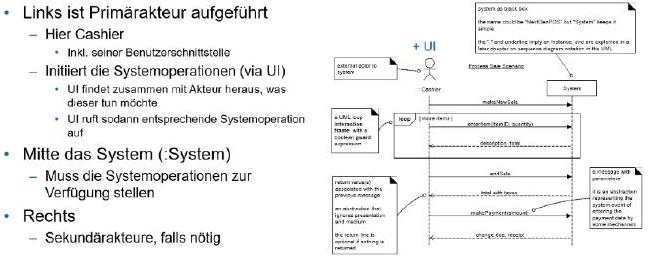
\includegraphics[width=\linewidth]{images/2024_12_29_0d1d7b5551ea1b4b41bdg-06}
\end{concept}

\begin{KR}{SSD Erstellung}
\begin{enumerate}
    \item Use Case als Grundlage wählen
    \item Akteur und System identifizieren
    \item Methodenaufrufe definieren:
    \begin{itemize}
        \item Namen aussagekräftig wählen
        \item Parameter festlegen
        \item Rückgabewerte bestimmen
    \end{itemize}
    \item Zeitliche Abfolge modellieren
    \item Optional: Externe Systeme einbinden
\end{enumerate}
\end{KR}

\begin{example}
\textbf{Aufgabe:} Erstellen Sie einen fully-dressed Use Case für ein Online-Bibliothekssystem. Fokus: "Buch ausleihen"

\textbf{Lösung:}
\begin{itemize}
    \item \textbf{Umfang:} Online-Bibliothekssystem
    \item \textbf{Primärakteur:} Bibliotheksnutzer
    \item \textbf{Stakeholder:} 
    \begin{itemize}
        \item Bibliotheksnutzer: Möchte Buch einfach ausleihen
        \item Bibliothek: Korrekte Erfassung der Ausleihe
    \end{itemize}
    \item \textbf{Vorbedingung:} Nutzer ist eingeloggt
    \item \textbf{Standardablauf:}
    \begin{enumerate}
        \item Nutzer sucht Buch
        \item System zeigt Verfügbarkeit
        \item Nutzer wählt Ausleihe
        \item System prüft Ausleihberechtigung
        \item System registriert Ausleihe
        \item System zeigt Bestätigung
    \end{enumerate}
    \item \textbf{Erweiterungen:}
    \begin{itemize}
        \item 2a: Buch nicht verfügbar
        \item 4a: Keine Ausleihberechtigung
    \end{itemize}
\end{itemize}
\end{example}

	\raggedcolumns
	\pagebreak
    \input{02_domänenmodellierung_new.tex}
	\raggedcolumns
	\pagebreak
    \section{Softwarearchitektur und Design}

\begin{concept}{Überblick Softwareentwicklung}\\
Die Entwicklung von Software erfolgt in verschiedenen Ebenen:
\begin{itemize}
    \item Business Analyse (Domänenmodell, Requirements)
    \item Architektur (Logische Struktur)
    \item Entwicklung (Konkrete Umsetzung)
\end{itemize}
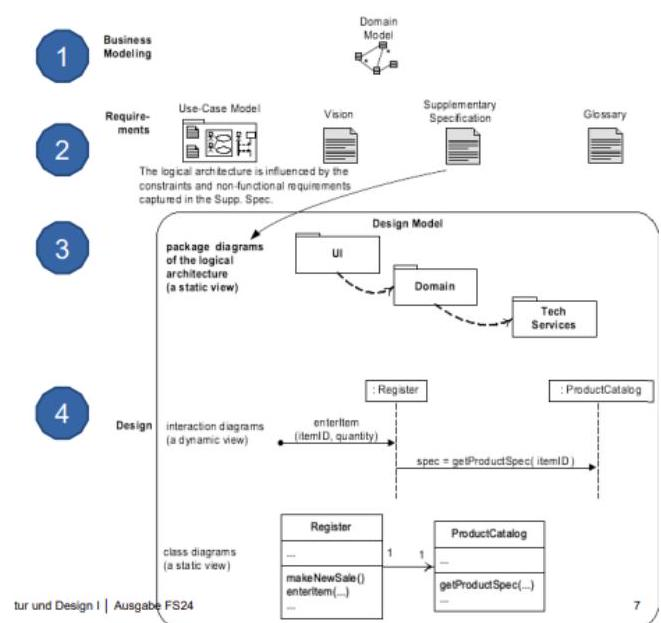
\includegraphics[width=0.9\linewidth]{images/2024_12_29_0d1d7b5551ea1b4b41bdg-07(2)}
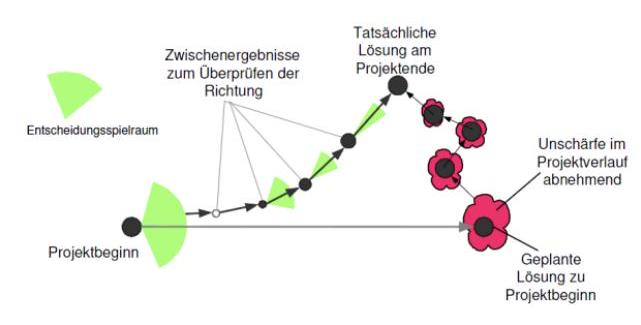
\includegraphics[width=0.9\linewidth]{images/2024_12_29_0d1d7b5551ea1b4b41bdg-08(1)}
\end{concept}

\begin{definition}{Softwarearchitektur}\\
Die Architektur definiert:
\begin{itemize}
    \item Grundlegende Strukturen und Komponenten
    \item Heutige und zukünftige Anforderungen
    \item Weiterentwicklungsmöglichkeiten
    \item Beziehungen zur Umgebung
\end{itemize}
\end{definition}

\begin{concept}{Architekturanalyse}\\
Die Analyse erfolgt iterativ mit den Anforderungen:
\begin{itemize}
    \item Analyse funktionaler und nicht-funktionaler Anforderungen
    \item Abstimmung mit Stakeholdern
    \item Kontinuierliche Weiterentwicklung
\end{itemize}
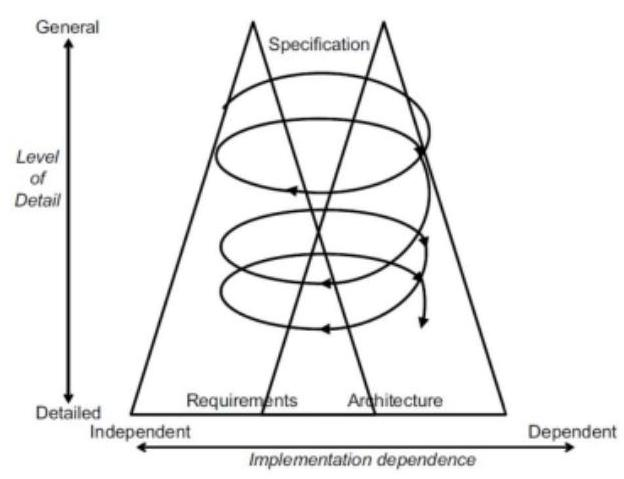
\includegraphics[width=0.9\linewidth]{images/2024_12_29_0d1d7b5551ea1b4b41bdg-08}
\end{concept}

\begin{theorem}{ISO 25010 vs FURPS+}\\
\textbf{ISO 25010:}
\begin{itemize}
    \item Hierarchische Struktur für nicht-funktionale Anforderungen
    \item Definierte Hauptcharakteristiken und Subcharakteristiken
    \item Messbare Metriken für jede Anforderung
    \item Präzise Formulierung und Verifikation
\end{itemize}

\textbf{FURPS+:}
\begin{itemize}
    \item Functionality (Funktionalität)
    \item Usability (Benutzbarkeit)
    \item Reliability (Zuverlässigkeit)
    \item Performance (Leistung)
    \item Supportability (Wartbarkeit)
    \item + (Implementation, Interface, Operations, Packaging, Legal)
\end{itemize}
\end{theorem}

\begin{concept}{Modulkonzept}\\
Ein Modul (Baustein, Komponente) wird bewertet nach:
\begin{itemize}
    \item \textbf{Kohäsion:} Innerer Zusammenhang
    \item \textbf{Kopplung:} Externe Abhängigkeiten
\end{itemize}

\textbf{Eigenschaften:}
\begin{itemize}
    \item Autarkes Teilsystem
    \item Minimale externe Schnittstellen
    \item Enthält alle benötigten Funktionen/Daten
    \item Verschiedene Formen: Paket, Library, Service
\end{itemize}
\end{concept}

\begin{concept}{Architektursichten}\\
Das N+1 View Model beschreibt verschiedene Perspektiven:
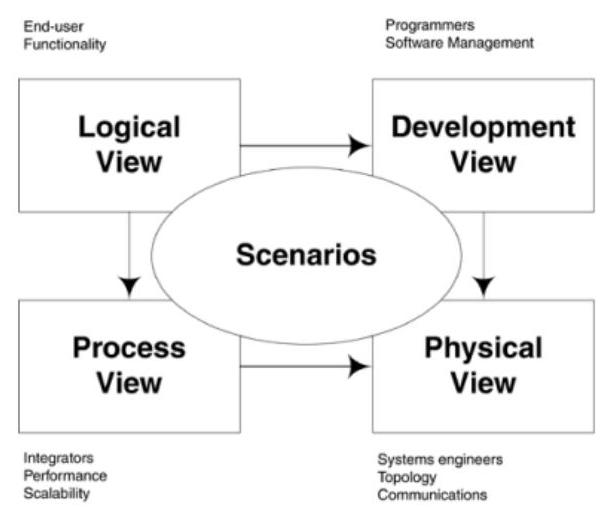
\includegraphics[width=0.9\linewidth]{images/2024_12_29_0d1d7b5551ea1b4b41bdg-09}

\textbf{UML-Paketdiagramm:}
\begin{itemize}
    \item Definition von Teilsystemen
    \item Gruppierung von Elementen
    \item Abhängigkeiten zwischen Paketen
\end{itemize}
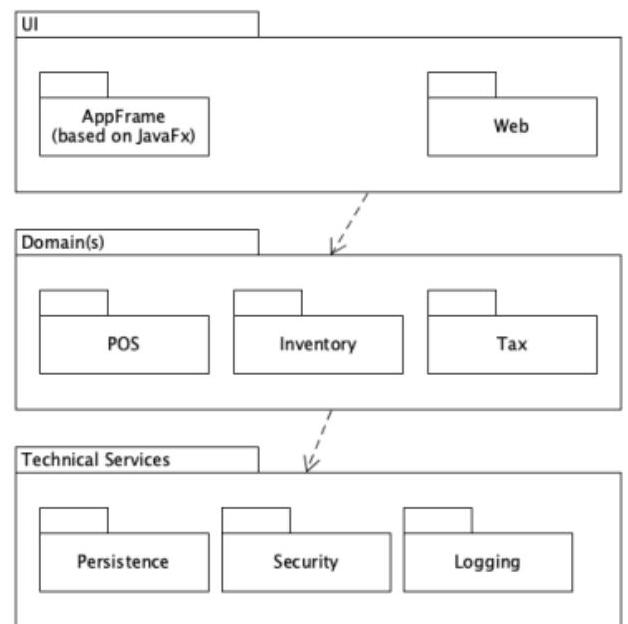
\includegraphics[width=0.9\linewidth]{images/2024_12_29_0d1d7b5551ea1b4b41bdg-09(1)}
\end{concept}

\subsubsection{UML-Modellierung}

\begin{KR}{Statische vs. Dynamische Modelle}\\
\textbf{Statische Modelle (Struktur):}
\begin{itemize}
    \item UML-Klassendiagramm
    \item Fokus auf Pakete, Klassen, Attribute
    \item Keine Methodenimplementierung
\end{itemize}

\textbf{Dynamische Modelle (Verhalten):}
\begin{itemize}
    \item UML-Interaktionsdiagramme
    \item Fokus auf Logik und Verhalten
    \item Implementierung der Methoden
\end{itemize}
\end{KR}

\begin{definition}{UML-Diagrammtypen}\\
\textbf{1. Klassendiagramm:}
\begin{itemize}
    \item Klassen und aktive Klassen
    \item Attribute und Operationen
    \item Sichtbarkeiten und Beziehungen
    \item Interfaces und Realisierungen
\end{itemize}

\textbf{2. Sequenzdiagramm:}
\begin{itemize}
    \item Lebenslinien und Nachrichten
    \item Synchrone/Asynchrone Kommunikation
    \item Aktivierung und Deaktivierung
    \item Alternative Abläufe
\end{itemize}

\textbf{3. Zustandsdiagramm:}
\begin{itemize}
    \item Zustände und Übergänge
    \item Start- und Endzustände
    \item Composite States
    \item Historie und Parallelität
\end{itemize}

\textbf{4. Aktivitätsdiagramm:}
\begin{itemize}
    \item Aktionen und Aktivitäten
    \item Kontroll- und Datenflüsse
    \item Verzweigungen und Zusammenführungen
    \item Partitionen (Swimlanes)
\end{itemize}
\end{definition}

\begin{concept}{Responsibility Driven Design (RDD)}\\
Design basierend auf Verantwortlichkeiten:
\begin{itemize}
    \item Klassenentwurf nach Rollen
    \item Kollaborationsbeziehungen
    \item Implementierung durch Attribute/Methoden
    \item Anwendbar auf allen Ebenen
\end{itemize}
\end{concept}

\begin{theorem}{GRASP Prinzipien}\\
General Responsibility Assignment Software Patterns:
\begin{itemize}
    \item \textbf{Information Expert:} Verantwortung basierend auf Information
    \item \textbf{Creator:} Objekterstellung bei starker Beziehung
    \item \textbf{Controller:} Zentrale Steuerungslogik
    \item \textbf{Low Coupling:} Minimale Abhängigkeiten
    \item \textbf{High Cohesion:} Starker innerer Zusammenhang
    \item \textbf{Polymorphism:} Flexibilität durch Schnittstellen
    \item \textbf{Pure Fabrication:} Künstliche Klassen für besseres Design
    \item \textbf{Indirection:} Vermittler für Flexibilität
    \item \textbf{Protected Variations:} Kapselung von Änderungen
\end{itemize}
\end{theorem}

\begin{example}{Architekturentwurf}
\textbf{Aufgabe:} Entwerfen Sie die grundlegende Architektur für ein Online-Banking-System.

\textbf{Lösung:}
\begin{itemize}
    \item \textbf{Anforderungsanalyse:}
    \begin{itemize}
        \item Sicherheit (ISO 25010)
        \item Performance (FURPS+)
        \item Skalierbarkeit
    \end{itemize}
    
    \item \textbf{Architekturentscheidungen:}
    \begin{itemize}
        \item Mehrschichtige Architektur
        \item Microservices für Skalierbarkeit
        \item Sicherheitsschicht
    \end{itemize}
    
    \item \textbf{Module:}
    \begin{itemize}
        \item Authentifizierung
        \item Transaktionen
        \item Kontoführung
    \end{itemize}
\end{itemize}
\end{example}

\begin{KR}{Architekturentwurf}
\textbf{Schritte:}
\begin{enumerate}
    \item Anforderungen analysieren
    \item Architekturstil wählen
    \item Module identifizieren
    \item Schnittstellen definieren
    \item Mit Stakeholdern abstimmen
\end{enumerate}

\textbf{Qualitätskriterien:}
\begin{itemize}
    \item Änderbarkeit
    \item Wartbarkeit
    \item Erweiterbarkeit
    \item Testbarkeit
\end{itemize}
\end{KR}
	\raggedcolumns
	\pagebreak
    \section{Use Case Realisation}

\begin{concept}{Use Case Realization}\\
Die Umsetzung von Use Cases erfolgt durch:
\begin{itemize}
    \item Detaillierte Szenarien aus den Use Cases
    \item Systemantworten müssen realisiert werden
    \item UI statt System im SSD
    \item Systemoperationen sind die zu implementierenden Elemente
\end{itemize}
\end{concept}

\begin{definition}{UML im Implementierungsprozess}\\
UML dient als:
\begin{itemize}
    \item Zwischenschritt bei wenig Erfahrung
    \item Kompakter Ersatz für Programmiercode
    \item Kommunikationsmittel (auch für Nicht-Techniker)
\end{itemize}
\end{definition}

\begin{KR}{Vorgehen bei der Use Case Realization}\\
\textbf{1. Vorbereitung:}
\begin{itemize}
    \item Use Case auswählen und SSD ableiten
    \item Systemoperation identifizieren
    \item Operation Contract erstellen/prüfen
\end{itemize}

\textbf{2. Analyse:}
\begin{itemize}
    \item Aktuellen Code/Dokumentation analysieren
    \item DCD überprüfen/aktualisieren
    \item Vergleich mit Domänenmodell
    \item Neue Klassen gemäß Domänenmodell erstellen
\end{itemize}

\textbf{3. Realisierung:}
\begin{itemize}
    \item Controller Klasse bestimmen
    \item Zu verändernde Klassen festlegen
    \item Weg zu diesen Klassen festlegen:
    \begin{itemize}
        \item Parameter für Wege definieren
        \item Klassen bei Bedarf erstellen
        \item Verantwortlichkeiten zuweisen
        \item Verschiedene Varianten evaluieren
    \end{itemize}
    \item Veränderungen implementieren
    \item Review durchführen
\end{itemize}
\end{KR}

\begin{example}{Use Case Realization: Verkauf abwickeln}
\textbf{1. Vorbereitung:}
\begin{itemize}
    \item \textbf{Use Case:} Verkauf abwickeln
    \item \textbf{Systemoperation:} makeNewSale()
    \item \textbf{Contract:} Neue Sale-Instanz wird erstellt
\end{itemize}

\textbf{2. Analyse:}
\begin{itemize}
    \item \textbf{Klassen:} Register, Sale
    \item \textbf{DCD:} Beziehung Register-Sale prüfen
    \item \textbf{Neue Klassen:} Payment, SaleLineItem
\end{itemize}

\textbf{3. Implementierung:}
\begin{itemize}
    \item Register als Controller
    \item Sale-Klasse erweitern
    \item Beziehungen implementieren
\end{itemize}
\end{example}

\begin{KR}{Typische Implementierungsfehler vermeiden}\\
\begin{itemize}
    \item \textbf{Architekturverletzungen:}
    \begin{itemize}
        \item Schichtentrennung beachten
        \item Abhängigkeiten richtig setzen
    \end{itemize}
    
    \item \textbf{GRASP-Verletzungen:}
    \begin{itemize}
        \item Information Expert beachten
        \item Creator Pattern richtig anwenden
        \item High Cohesion erhalten
    \end{itemize}
    
    \item \textbf{Testbarkeit:}
    \begin{itemize}
        \item Klassen isoliert testbar halten
        \item Abhängigkeiten mockbar gestalten
    \end{itemize}
\end{itemize}
\end{KR}

	\raggedcolumns
	\pagebreak
    \section{Design Patterns}

\begin{concept}{Grundlagen Design Patterns}\\
Bewährte Lösungsmuster für wiederkehrende Probleme:
\begin{itemize}
    \item Beschleunigen Entwicklung durch vorgefertigte Lösungen
    \item Verbessern Kommunikation im Team
    \item Bieten Balance zwischen Flexibilität und Komplexität
    \item \textbf{Wichtig:} Design Patterns sind kein Selbstzweck
\end{itemize}
\end{concept}

\subsection{Grundlegende Design Patterns}

\begin{definition}{Adapter Pattern}\\
\textbf{Problem:} Inkompatible Schnittstellen
\begin{itemize}
    \item Objekte mit unterschiedlichen Interfaces sollen zusammenarbeiten
    \item Externe Dienste sollen austauschbar sein
\end{itemize}
\textbf{Lösung:} Adapter-Klasse als Vermittler
\end{definition}

\begin{definition}{Simple Factory Pattern}\\
\textbf{Problem:} Komplexe Objekterzeugung
\begin{itemize}
    \item Objekterzeugung erfordert viele Schritte
    \item Konfiguration bei Erzeugung notwendig
\end{itemize}
\textbf{Lösung:} Eigene Klasse für Objekterzeugung
\end{definition}

\begin{definition}{Singleton Pattern}\\
\textbf{Problem:} Genau eine Instanz benötigt
\begin{itemize}
    \item Globaler Zugriffspunkt notwendig
    \item Mehrfachinstanzierung verhindern
\end{itemize}
\textbf{Lösung:} Statische Instanz mit privater Erzeugung
\end{definition}

\begin{definition}{Dependency Injection Pattern}\\
\textbf{Problem:} Abhängigkeiten zu anderen Objekten
\begin{itemize}
    \item Lose Kopplung erwünscht
    \item Flexibilität bei Abhängigkeiten
\end{itemize}
\textbf{Lösung:} Abhängigkeiten werden von außen injiziert
\end{definition}

\begin{definition}{Proxy Pattern}\\
\textbf{Problem:} Zugriffskontrolle auf Objekte
\begin{itemize}
    \item Verzögertes Laden
    \item Zugriffsbeschränkungen
    \item Netzwerkkommunikation
\end{itemize}
\textbf{Lösung:} Stellvertreterobjekt mit gleichem Interface
\begin{itemize}
    \item \textbf{Remote Proxy:} Für entfernte Objekte
    \item \textbf{Virtual Proxy:} Für spätes Laden
    \item \textbf{Protection Proxy:} Für Zugriffsschutz
\end{itemize}
\end{definition}

\begin{definition}{Chain of Responsibility Pattern}\\
\textbf{Problem:} Unklare Zuständigkeit für Anfragen
\begin{itemize}
    \item Mehrere mögliche Handler
    \item Zuständigkeit erst zur Laufzeit klar
\end{itemize}
\textbf{Lösung:} Verkettete Handler-Objekte
\end{definition}

\subsection{Erweiterte Design Patterns}

\begin{definition}{Decorator Pattern}\\
\textbf{Problem:} Dynamische Erweiterung von Objekten
\begin{itemize}
    \item Zusätzliche Verantwortlichkeiten
    \item Nur für einzelne Objekte
\end{itemize}
\textbf{Lösung:} Wrapper-Objekt mit gleichem Interface
\end{definition}

\begin{definition}{Observer Pattern}\\
\textbf{Problem:} Abhängige Objekte aktualisieren
\begin{itemize}
    \item Lose Kopplung erwünscht
    \item Typ des Empfängers unbekannt
\end{itemize}
\textbf{Lösung:} Observer-Interface für Benachrichtigungen
\end{definition}

\begin{definition}{Strategy Pattern}\\
\textbf{Problem:} Austauschbare Algorithmen
\begin{itemize}
    \item Verschiedene Implementierungen
    \item Zur Laufzeit wechselbar
\end{itemize}
\textbf{Lösung:} Interface für Algorithmus-Klassen
\end{definition}

\begin{definition}{Composite Pattern}\\
\textbf{Problem:} Baumstrukturen verwalten
\begin{itemize}
    \item Einheitliche Behandlung
    \item Teil-Ganzes Hierarchie
\end{itemize}
\textbf{Lösung:} Gemeinsames Interface für Container und Inhalt
\end{definition}

\begin{KR}{Design Pattern Auswahl}\\
\textbf{Schritt 1: Problem analysieren}
\begin{itemize}
    \item Art des Problems identifizieren
    \item Anforderungen klar definieren
    \item Kontext verstehen
\end{itemize}

\textbf{Schritt 2: Pattern evaluieren}
\begin{itemize}
    \item Passende Patterns suchen
    \item Vor- und Nachteile abwägen
    \item Komplexität bewerten
\end{itemize}

\textbf{Schritt 3: Implementation planen}
\begin{itemize}
    \item Klassenstruktur entwerfen
    \item Schnittstellen definieren
    \item Anpassungen vornehmen
\end{itemize}
\end{KR}



	\raggedcolumns
	\pagebreak
	\section{Implementation, Refactoring und Testing}

\subsection{Design to Code}

\begin{concept}{Umsetzungsstrategien}
\textbf{Code-Driven Development:}
\begin{itemize}
    \item Direkte Implementierung der Klassen
    \item Nachträgliches Testing
\end{itemize}

\textbf{Test-Driven Development (TDD):}
\begin{itemize}
    \item Tests vor Implementation
    \item Red-Green-Refactor Zyklus
\end{itemize}

\textbf{Behavior-Driven Development (BDD):}
\begin{itemize}
    \item Testbeschreibung aus Anwendersicht
    \item Gherkin-Syntax für Szenarios
\end{itemize}
\end{concept}

\begin{KR}{Implementation Grundsätze}
\textbf{1. Code-Guidelines:}
\begin{itemize}
    \item Einheitliche Formatierung
    \item Klare Namenskonventionen
    \item Dokumentationsrichtlinien
\end{itemize}

\textbf{2. Fehlerbehandlung:}
\begin{itemize}
    \item Exceptions statt Fehlercodes
    \item Sinnvolle Error Messages
    \item Logging-Strategie
\end{itemize}

\textbf{3. Namensgebung:}
\begin{itemize}
    \item Aussagekräftige Namen
    \item Konsistente Begriffe
    \item Domain-Driven Naming
\end{itemize}
\end{KR}

\subsection{Refactoring}

\begin{definition}{Refactoring Grundlagen}
Strukturierte Verbesserung des Codes ohne Änderung des externen Verhaltens:
\begin{itemize}
    \item Kleine, kontrollierte Schritte
    \item Erhaltung der Funktionalität 
    \item Verbesserung der Codequalität und interner Struktur
    \item Ziel: Bessere Wartbarkeit und Erweiterbarkeit
\end{itemize}
\end{definition}

\begin{definition}{Code Smells}
Anzeichen für mögliche Probleme im Code:
\begin{itemize}
    \item Duplizierter Code
    \item Lange Methoden
    \item Klassen mit vielen Instanzvariablen
    \item Klassen mit sehr viel Code
    \item Auffällig ähnliche Unterklassen
    \item Keine Interfaces
    \item Hohe Kopplung zwischen Klassen
\end{itemize}
\end{definition}

\begin{KR}{Refactoring Patterns}
\textbf{1. Extract Method}
\begin{itemize}
    \item Code in eigene Methode auslagern
    \item Verbessert Lesbarkeit und Wiederverwendbarkeit
    \item Reduziert Duplikation
\end{itemize}

\textbf{2. Move Method/Field}
\begin{itemize}
    \item Methode/Feld in andere Klasse verschieben
    \item Verbessert Kohäsion
    \item Folgt Information Expert
\end{itemize}

\textbf{3. Extract Class}
\begin{itemize}
    \item Teil einer Klasse in neue Klasse auslagern
    \item Trennt Verantwortlichkeiten
    \item Erhöht Kohäsion
\end{itemize}

\textbf{4. Rename Method/Class/Variable}
\begin{itemize}
    \item Bessere Namen für besseres Verständnis
    \item Dokumentiert Zweck
    \item Erleichtert Wartung
\end{itemize}
\end{KR}

\subsection{Testing}

\begin{concept}{Teststufen}
\begin{itemize}
\item \textbf{Unit Tests:} 
\begin{itemize}
    \item Einzelne Komponenten
    \item Isolation durch Mocks/Stubs
    \item Schnelle Ausführung
\end{itemize}

\item \textbf{Integrationstests:} 
\begin{itemize} 
    \item Zusammenspiel mehrerer Komponenten
    \item Schnittstellen-Tests
    \item Externe Systeme
\end{itemize}

\item \textbf{Systemtests:} 
\begin{itemize}
    \item End-to-End Szenarien
    \item Nicht-funktionale Anforderungen
\end{itemize}

\item \textbf{Abnahmetests:} 
\begin{itemize}
    \item Gegen Kundenanforderungen
    \item User Acceptance Testing (UAT)
\end{itemize}
\end{itemize}
\end{concept}

\begin{KR}{Testdesign}
\textbf{1. Funktionaler Test (Black-Box)}
\begin{itemize}
    \item Test aus Benutzersicht
    \item Ohne Codekenntnis
    \item Fokus auf Input/Output
\end{itemize}

\textbf{2. Strukturbezogener Test (White-Box)}
\begin{itemize}
    \item Test mit Codekenntnis
    \item Code Coverage
    \item Pfadtests
\end{itemize}

\textbf{3. Änderungsbezogener Test}
\begin{itemize}
    \item Regressionstest
    \item Verifizierung von Änderungen
    \item Sicherstellung der Gesamtfunktionalität
\end{itemize}
\end{KR}

\begin{definition}{Testbegriffe}
\begin{itemize}
    \item \textbf{Testling/Testobjekt:} Das zu testende Element
    \item \textbf{Fehler:} Fehler des Entwicklers bei der Implementation
    \item \textbf{Fehlerwirkung/Bug:} Abweichung vom spezifizierten Verhalten
    \item \textbf{Testfall:} Spezifische Testkonfiguration mit Testdaten
    \item \textbf{Testtreiber:} Programm zur Testausführung
\end{itemize}
\end{definition}

%todo: Add examples for:
% - Refactoring before/after
% - Unit test with mocks
% - Integration test setup
% - Test case design examples
	\raggedcolumns
	\pagebreak
    \section{Implementation, Refactoring und Testing}

\subsection{Von Design zu Code}

\begin{concept}{Implementierungsstrategien}\\
\textbf{1. Bottom-Up Entwicklung:}
\begin{itemize}
    \item Implementierung beginnt mit Basisbausteinen
    \item Schrittweise Integration zu größeren Komponenten
    \item \textbf{Vorteile:} Gründlich, solide Basis
    \item \textbf{Nachteile:} Spätes Feedback
\end{itemize}

\textbf{2. Agile Entwicklung:}
\begin{itemize}
    \item Inkrementelle Entwicklung in Sprints
    \item Kontinuierliche Integration und Auslieferung
    \item \textbf{Vorteile:} Flexibilität, schnelles Feedback
    \item \textbf{Nachteile:} Mögliche Restrukturierung nötig
\end{itemize}
\end{concept}

\begin{definition}{Entwicklungsansätze}\\
\textbf{Code-Driven Development (CDD):}
\begin{itemize}
    \item Direkte Implementierung der Klassen
    \item Nachträgliches Testing
\end{itemize}

\textbf{Test-Driven Development (TDD):}
\begin{itemize}
    \item Tests vor Implementation
    \item Red-Green-Refactor Zyklus
\end{itemize}

\textbf{Behavior-Driven Development (BDD):}
\begin{itemize}
    \item Testbeschreibung aus Anwendersicht
    \item Gherkin-Syntax für Szenarios
\end{itemize}
\end{definition}

\begin{KR}{Clean Code}\\
\textbf{1. Code-Guidelines:}
\begin{itemize}
    \item Einheitliche Formatierung
    \item Klare Namenskonventionen
    \item Dokumentationsrichtlinien
\end{itemize}

\textbf{2. Fehlerbehandlung:}
\begin{itemize}
    \item Exceptions statt Fehlercodes
    \item Sinnvolle Error Messages
    \item Logging-Strategie
\end{itemize}

\textbf{3. Namensgebung:}
\begin{itemize}
    \item Aussagekräftige Namen
    \item Konsistente Begriffe
    \item Domain-Driven Naming
\end{itemize}
\end{KR}

\begin{concept}{Laufzeit-Optimierung}\\
\textbf{Grundregeln:}
\begin{itemize}
    \item Zuerst messen, dann optimieren
    \item Performance-Profile nutzen
    \item Bottlenecks identifizieren
\end{itemize}

\textbf{Häufige Probleme:}
\begin{itemize}
    \item Datenbank-Zugriffe
    \item Ineffiziente Algorithmen
    \item Speicherlecks
\end{itemize}
\end{concept}

\subsection{Refactoring}

\begin{definition}{Refactoring Grundlagen}\\
Strukturierte Verbesserung des Codes ohne Änderung des externen Verhaltens:
\begin{itemize}
    \item Kleine, kontrollierte Schritte
    \item Erhaltung der Funktionalität
    \item Verbesserung der Codequalität
\end{itemize}
\end{definition}

\begin{KR}{Refactoring Durchführung}\\
\textbf{1. Code Smells identifizieren:}
\begin{itemize}
    \item Duplizierter Code
    \item Lange Methoden
    \item Große Klassen
    \item Hohe Kopplung
\end{itemize}

\textbf{2. Refactoring durchführen:}
\begin{itemize}
    \item Tests sicherstellen
    \item Änderungen vornehmen
    \item Tests ausführen
\end{itemize}

\textbf{3. Patterns anwenden:}
\begin{itemize}
    \item Extract Method
    \item Move Method
    \item Rename
    \item Introduce Variable
\end{itemize}
\end{KR}



\subsection{Testing}

\begin{definition}{Testarten}\\
\textbf{Nach Sicht:}
\begin{itemize}
    \item \textbf{Black-Box:} Funktionaler Test ohne Codekenntnis
    \item \textbf{White-Box:} Strukturbezogener Test mit Codekenntnis
\end{itemize}

\textbf{Nach Umfang:}
\begin{itemize}
    \item \textbf{Unit-Tests:} Einzelne Komponenten
    \item \textbf{Integrationstests:} Zusammenspiel
    \item \textbf{Systemtests:} Gesamtsystem
    \item \textbf{Akzeptanztests:} Kundenanforderungen
\end{itemize}
\end{definition}

\begin{KR}{Testentwicklung}\\
\textbf{1. Testfall definieren:}
\begin{itemize}
    \item Vorbedingungen festlegen
    \item Testdaten vorbereiten
    \item Erwartetes Ergebnis definieren
\end{itemize}

\textbf{2. Test implementieren:}
\begin{itemize}
    \item Setup vorbereiten
    \item Testlogik schreiben
    \item Assertions definieren
\end{itemize}

\textbf{3. Test ausführen:}
\begin{itemize}
    \item Automatisiert ausführen
    \item Ergebnisse prüfen
    \item Dokumentation erstellen
\end{itemize}
\end{KR}



	\raggedcolumns
	\pagebreak
	[Previous content until initial definitions remains unchanged]

\begin{example}{Prüfungsaufgabe: Architekturstil-Analyse}
\textbf{Szenario:}
Ein Messaging-System soll entwickelt werden, das folgende Anforderungen erfüllt:
\begin{itemize}
    \item Hohe Skalierbarkeit
    \item Keine zentrale Komponente (Single Point of Failure)
    \item Direkter Nachrichtenaustausch zwischen Nutzern
    \item Offline-Fähigkeit
\end{itemize}

\textbf{Analysieren Sie die Architekturstile:}

\textbf{1. Client-Server}
\begin{itemize}
    \item \textbf{Vorteile:}
    \begin{itemize}
        \item Zentrale Verwaltung
        \item Einfache Konsistenzsicherung
    \end{itemize}
    \item \textbf{Nachteile:}
    \begin{itemize}
        \item Single Point of Failure
        \item Skalierungsprobleme
    \end{itemize}
\end{itemize}

\textbf{2. Peer-to-Peer}
\begin{itemize}
    \item \textbf{Vorteile:}
    \begin{itemize}
        \item Keine zentrale Komponente
        \item Direkte Kommunikation
        \item Gute Skalierbarkeit
    \end{itemize}
    \item \textbf{Nachteile:}
    \begin{itemize}
        \item Komplexe Konsistenzsicherung
        \item Schwierige Verwaltung
    \end{itemize}
\end{itemize}

\textbf{Empfehlung:} Peer-to-Peer mit hybriden Elementen
\end{example}

\begin{KR}{Verteilungsprobleme analysieren}
\textbf{1. Probleme identifizieren}
\begin{itemize}
    \item \textbf{Netzwerk:}
    \begin{itemize}
        \item Latenz
        \item Bandbreite
        \item Ausfälle
    \end{itemize}
    \item \textbf{Daten:}
    \begin{itemize}
        \item Konsistenz
        \item Replikation
        \item Synchronisation
    \end{itemize}
    \item \textbf{System:}
    \begin{itemize}
        \item Skalierung
        \item Verfügbarkeit
        \item Wartbarkeit
    \end{itemize}
\end{itemize}

\textbf{2. Lösungsstrategien entwickeln}
\begin{itemize}
    \item \textbf{Netzwerk:}
    \begin{itemize}
        \item Caching
        \item Compression
        \item Redundanz
    \end{itemize}
    \item \textbf{Daten:}
    \begin{itemize}
        \item Eventual Consistency
        \item Master-Slave Replikation
        \item Konfliktauflösung
    \end{itemize}
    \item \textbf{System:}
    \begin{itemize}
        \item Load Balancing
        \item Service Discovery
        \item Circuit Breaker
    \end{itemize}
\end{itemize}
\end{KR}

\begin{example}{Typische Prüfungsaufgabe: CAP-Theorem}
\textbf{Aufgabe:}
Analysieren Sie für ein verteiltes Datenbanksystem die Auswirkungen des CAP-Theorems.

\textbf{CAP-Theorem Komponenten:}
\begin{itemize}
    \item \textbf{Consistency:} Alle Knoten sehen dieselben Daten
    \item \textbf{Availability:} Jede Anfrage erhält eine Antwort
    \item \textbf{Partition Tolerance:} System funktioniert trotz Netzwerkausfällen
\end{itemize}

\textbf{Analyse der Trade-offs:}
\begin{itemize}
    \item \textbf{CA-System:}
    \begin{itemize}
        \item Hohe Konsistenz und Verfügbarkeit
        \item Keine Netzwerkpartitionierung möglich
        \item Beispiel: Traditionelle RDBMS
    \end{itemize}
    \item \textbf{CP-System:}
    \begin{itemize}
        \item Konsistenz und Partitionstoleranz
        \item Eingeschränkte Verfügbarkeit
        \item Beispiel: MongoDB
    \end{itemize}
    \item \textbf{AP-System:}
    \begin{itemize}
        \item Verfügbarkeit und Partitionstoleranz
        \item Eventual Consistency
        \item Beispiel: Cassandra
    \end{itemize}
\end{itemize}
\end{example}

\begin{KR}{Verteilte System-Design}
\textbf{1. Anforderungsanalyse}
\begin{itemize}
    \item \textbf{Funktional:}
    \begin{itemize}
        \item Kernfunktionalitäten
        \item Datenmodell
        \item Schnittstellen
    \end{itemize}
    \item \textbf{Nicht-funktional:}
    \begin{itemize}
        \item Skalierbarkeit
        \item Verfügbarkeit
        \item Latenz
    \end{itemize}
\end{itemize}

\textbf{2. Architekturentscheidungen}
\begin{itemize}
    \item \textbf{Kommunikation:}
    \begin{itemize}
        \item Synchron vs. Asynchron
        \item Push vs. Pull
        \item Protokollwahl
    \end{itemize}
    \item \textbf{Datenmanagement:}
    \begin{itemize}
        \item Sharding
        \item Replikation
        \item Caching
    \end{itemize}
\end{itemize}

\textbf{3. Implementierungsaspekte}
\begin{itemize}
    \item \textbf{Fehlerbehandlung:}
    \begin{itemize}
        \item Retry-Strategien
        \item Fallbacks
        \item Monitoring
    \end{itemize}
    \item \textbf{Sicherheit:}
    \begin{itemize}
        \item Authentifizierung
        \item Verschlüsselung
        \item Autorisierung
    \end{itemize}
\end{itemize}
\end{KR}

[Previous content about middleware and error sources remains]
	\raggedcolumns
	\pagebreak
    \section{Verteilte Systeme}

\begin{definition}{Verteiltes System}\\
Ein Netzwerk aus autonomen Computern und Softwarekomponenten, die als einheitliches System erscheinen:
\begin{itemize}
    \item Autonome Knoten und Komponenten
    \item Netzwerkverbindung
    \item Erscheint als ein System
\end{itemize}
\end{definition}

\begin{concept}{Charakteristika verteilter Systeme}\\
Typische Merkmale moderner verteilter Systeme:
\begin{itemize}
    \item \textbf{Skalierbarkeit:} Oft sehr große Systeme
    \item \textbf{Datenorientierung:} Zentrale Datenbanken
    \item \textbf{Interaktivität:} GUI und Batch-Verarbeitung
    \item \textbf{Nebenläufigkeit:} Parallele Benutzerinteraktionen
    \item \textbf{Konsistenz:} Hohe Anforderungen an Datenkonsistenz
\end{itemize}
\end{concept}

\begin{theorem}{Grundlegende Konzepte}\\
\textbf{1. Kommunikation:}
\begin{itemize}
    \item Remote Procedure Calls (RPC)
    \item Message Queuing
    \item Publish-Subscribe-Systeme
\end{itemize}

\textbf{2. Fehlertoleranz:}
\begin{itemize}
    \item Replikation von Komponenten
    \item Failover-Mechanismen
    \item Fehlererkennung und -behandlung
\end{itemize}

\textbf{3. Fehlersemantik:}
\begin{itemize}
    \item Konsistenzgarantien
    \item Recovery-Verfahren
    \item Kompensationsmechanismen
\end{itemize}
\end{theorem}

\begin{concept}{Architekturmuster}\\
Grundlegende Architekturstile für verteilte Systeme:
\begin{itemize}
    \item \textbf{Client-Server:} Zentraler Server, multiple Clients
    \item \textbf{Peer-to-Peer:} Gleichberechtigte Knoten
    \item \textbf{Publish-Subscribe:} Event-basierte Kommunikation
\end{itemize}
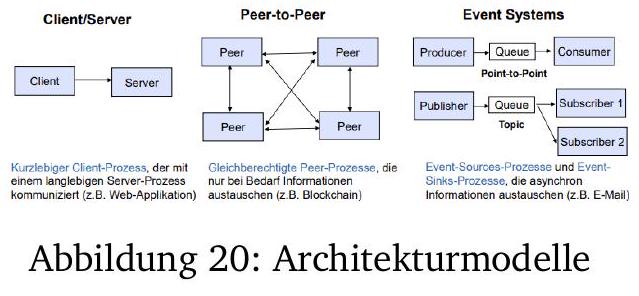
\includegraphics[width=0.9\linewidth]{images/2024_12_29_0d1d7b5551ea1b4b41bdg-18}
\end{concept}

\begin{KR}{Entwurf verteilter Systeme}\\
\textbf{1. Systemanalyse}
\begin{itemize}
    \item Anforderungen identifizieren
    \item Verteilungsaspekte analysieren
    \item Konsistenzanforderungen definieren
\end{itemize}

\textbf{2. Architekturentscheidungen}
\begin{itemize}
    \item Architekturstil wählen
    \item Kommunikationsmuster festlegen
    \item Fehlertoleranzstrategie definieren
\end{itemize}

\textbf{3. Technologieauswahl}
\begin{itemize}
    \item Middleware evaluieren
    \item Protokolle bestimmen
    \item Werkzeuge auswählen
\end{itemize}
\end{KR}

\begin{concept}{Middleware-Technologien}\\
Gängige Technologien für verteilte Systeme:
\begin{itemize}
    \item \textbf{Message Broker:} 
    \begin{itemize}
        \item Apache Kafka
        \item RabbitMQ
    \end{itemize}
    \item \textbf{RPC Frameworks:}
    \begin{itemize}
        \item gRPC
        \item CORBA
    \end{itemize}
    \item \textbf{Web Services:}
    \begin{itemize}
        \item RESTful APIs
        \item GraphQL
    \end{itemize}
\end{itemize}
\end{concept}



\begin{KR}{Typische Fehlerquellen}\\
\textbf{1. Netzwerkfehler}
\begin{itemize}
    \item Verbindungsabbrüche
    \item Timeouts
    \item Partitionierung
\end{itemize}

\textbf{2. Konsistenzprobleme}
\begin{itemize}
    \item Race Conditions
    \item Veraltete Daten
    \item Lost Updates
\end{itemize}

\textbf{3. Skalierungsprobleme}
\begin{itemize}
    \item Lastverteilung
    \item Resource-Management
    \item Bottlenecks
\end{itemize}

\textbf{Lösungsstrategien:}
\begin{itemize}
    \item Circuit Breaker Pattern
    \item Retry mit Exponential Backoff
    \item Idempotente Operationen
    \item Optimistic Locking
\end{itemize}
\end{KR}

	\raggedcolumns
	\pagebreak
	\subsection{Common Pitfalls und Best Practices}

\begin{concept}{Common Pitfalls in JPA Implementation}
\textbf{N+1 Problem:}
\begin{itemize}
    \item \textbf{Symptom:} Für jedes Objekt wird eine zusätzliche Query ausgeführt
    \item \textbf{Lösung:} Join Fetch oder Eager Loading strategisch einsetzen
\end{itemize}

\textbf{LazyInitializationException:}
\begin{itemize}
    \item \textbf{Symptom:} Zugriff auf lazy geladene Referenz außerhalb der Session
    \item \textbf{Lösung:} Transaktionen korrekt abgrenzen
\end{itemize}

\textbf{Bidirektionale Beziehungen:}
\begin{itemize}
    \item \textbf{Symptom:} Inkonsistente Objektzustände
    \item \textbf{Lösung:} Helper-Methoden für Beziehungspflege
\end{itemize}
\end{concept}

\begin{KR}{Best Practices für Persistenz}
\textbf{1. Architektur-Ebene}
\begin{itemize}
    \item Repository für Datenzugriff
    \item Service für Geschäftslogik
    \item DTO für Datentransfer
\end{itemize}

\textbf{2. Entity Design}
\begin{itemize}
    \item Immutable wenn möglich
    \item Bean Validation nutzen
    \item Geschäftsregeln in Entity-Klassen
\end{itemize}

\textbf{3. Performance}
\begin{itemize}
    \item Caching Strategien
    \item Batch Processing
    \item Query Optimierung
\end{itemize}
\end{KR}

\subsection{Parent-Child Beziehungen}

\begin{concept}{Parent-Child Mapping}
\textbf{Implementationsaspekte:}
\begin{itemize}
    \item Cascade-Typen definieren
    \item Bidirektionale Navigation
    \item Lazy Loading konfigurieren
    \item Orphan Removal festlegen
\end{itemize}

\textbf{JPA Annotationen:}
\begin{itemize}
    \item @OneToMany / @ManyToOne
    \item @JoinColumn
    \item mappedBy Parameter
    \item fetch = FetchType.LAZY/EAGER
\end{itemize}
\end{concept}

\subsection{Repository Pattern}

\begin{concept}{Spring Data Repository}
\textbf{Vorteile:}
\begin{itemize}
    \item Standardisierte CRUD-Operationen
    \item Query-Methoden aus Methodennamen
    \item Paginierung und Sortierung
    \item Einfache Integration mit Spring
\end{itemize}

\textbf{Repository Hierarchie:}
\begin{itemize}
    \item Repository (Marker Interface)
    \item CrudRepository (Basis CRUD)
    \item PagingAndSortingRepository
    \item JpaRepository (JPA-spezifisch)
\end{itemize}
\end{concept}

\begin{KR}{Repository Design}
\textbf{1. Interface Definition}
\begin{itemize}
    \item Domänenspezifische Methoden
    \item Query-Methoden
    \item Custom Implementations
\end{itemize}

\textbf{2. Query Methoden}
\begin{itemize}
    \item Methodennamen-Konventionen
    \item @Query Annotation
    \item Native Queries
\end{itemize}

\textbf{3. Transaktionshandling}
\begin{itemize}
    \item @Transactional Annotation
    \item Isolation Level
    \item Propagation Rules
\end{itemize}
\end{KR}

\subsection{Performance Optimierung}

\begin{KR}{Optimierungsstrategien}
\textbf{1. Fetch-Strategien}
\begin{itemize}
    \item Lazy Loading als Default
    \item Joins für häufig benötigte Daten
    \item EntityGraphs für komplexe Szenarien
\end{itemize}

\textbf{2. Caching}
\begin{itemize}
    \item First-Level Cache (Session)
    \item Second-Level Cache
    \item Query Cache
\end{itemize}

\textbf{3. Batch-Verarbeitung}
\begin{itemize}
    \item Batch Inserts/Updates
    \item JDBC Batch Size
    \item Pagination für große Datensätze
\end{itemize}
\end{KR}

%todo: Add examples for:
% - Handling parent-child relationships
% - Repository implementation with Spring Data
% - Performance optimization scenarios
% - Common pitfall solutions

\begin{concept}{Transaktionsmanagement}
\textbf{ACID-Eigenschaften:}
\begin{itemize}
    \item Atomicity (Atomarität)
    \item Consistency (Konsistenz)
    \item Isolation (Isolation)
    \item Durability (Dauerhaftigkeit)
\end{itemize}

\textbf{Isolation Levels:}
\begin{itemize}
    \item READ\_UNCOMMITTED
    \item READ\_COMMITTED
    \item REPEATABLE\_READ
    \item SERIALIZABLE
\end{itemize}
\end{concept}
	\raggedcolumns
	\pagebreak
    \section{Persistenz}

\begin{concept}{Persistenz Grundlagen}
[Previous content remains the same...]
\end{concept}

\begin{example}{O/R-Mapping Probleme und Lösungen}
\begin{lstlisting}[language=Java]
// Problem 1: Vererbung
@Entity
@Inheritance(strategy = InheritanceType.JOINED)
public abstract class Payment {
    @Id private Long id;
    private BigDecimal amount;
}

@Entity
public class CreditCardPayment extends Payment {
    private String cardNumber;
    private String expiryDate;
}

// Problem 2: Beziehungen
@Entity
public class Order {
    @ManyToOne
    private Customer customer;
    
    @OneToMany(mappedBy = "order", cascade = CascadeType.ALL)
    private List<OrderItem> items;
}

// Problem 3: Value Objects
@Embeddable
public class Money {
    private BigDecimal amount;
    private Currency currency;
}
\end{lstlisting}
\end{example}

\begin{KR}{JDBC Best Practices}
\begin{lstlisting}[language=Java]
public class DatabaseUtils {
    // 1. Connection Pool verwenden
    private final DataSource dataSource;
    
    // 2. Try-with-resources fuer automatisches Schliessen
    public List<Customer> findCustomers(String name) {
        String sql = "SELECT * FROM customers WHERE name = ?";
        
        try (Connection conn = dataSource.getConnection();
             PreparedStatement stmt = conn.prepareStatement(sql)) {
            
            // 3. Prepared Statements gegen SQL-Injection
            stmt.setString(1, name);
            
            // 4. ResultSet verarbeiten
            try (ResultSet rs = stmt.executeQuery()) {
                List<Customer> customers = new ArrayList<>();
                while (rs.next()) {
                    customers.add(mapCustomer(rs));
                }
                return customers;
            }
        }
    }
    
    // 5. Mapping in separate Methode
    private Customer mapCustomer(ResultSet rs) 
            throws SQLException {
        Customer customer = new Customer();
        customer.setId(rs.getLong("id"));
        customer.setName(rs.getString("name"));
        return customer;
    }
}
\end{lstlisting}
\end{KR}

\begin{example}{DAO Pattern Implementation}
\begin{lstlisting}[language=Java]
// 1. DAO Interface
public interface CustomerDao {
    Customer findById(Long id);
    List<Customer> findByName(String name);
    void save(Customer customer);
    void delete(Customer customer);
}

// 2. JDBC Implementation
public class JdbcCustomerDao implements CustomerDao {
    private final DataSource dataSource;
    
    @Override
    public Customer findById(Long id) {
        String sql = "SELECT * FROM customers WHERE id = ?";
        try (Connection conn = dataSource.getConnection();
             PreparedStatement stmt = 
                 conn.prepareStatement(sql)) {
            stmt.setLong(1, id);
            try (ResultSet rs = stmt.executeQuery()) {
                if (rs.next()) {
                    return mapCustomer(rs);
                }
                return null;
            }
        }
    }
    
    @Override
    public void save(Customer customer) {
        if (customer.getId() == null) {
            insert(customer);
        } else {
            update(customer);
        }
    }
}

// 3. JPA Implementation
@Repository
public class JpaCustomerDao implements CustomerDao {
    @PersistenceContext
    private EntityManager em;
    
    @Override
    public Customer findById(Long id) {
        return em.find(Customer.class, id);
    }
    
    @Override
    @Transactional
    public void save(Customer customer) {
        if (customer.getId() == null) {
            em.persist(customer);
        } else {
            em.merge(customer);
        }
    }
}
\end{lstlisting}
\end{example}

\begin{example}{JPA Entity mit Beziehungen}
\begin{lstlisting}[language=Java]
@Entity
@Table(name = "orders")
public class Order {
    @Id
    @GeneratedValue(strategy = GenerationType.IDENTITY)
    private Long id;
    
    @ManyToOne(fetch = FetchType.LAZY)
    @JoinColumn(name = "customer_id")
    private Customer customer;
    
    @OneToMany(mappedBy = "order", 
               cascade = CascadeType.ALL,
               orphanRemoval = true)
    private List<OrderItem> items = new ArrayList<>();
    
    @Embedded
    private Address shippingAddress;
    
    @Enumerated(EnumType.STRING)
    private OrderStatus status;
    
    @Version
    private Long version;
    
    // Hilfsmethoden fuer Beziehungsverwaltung
    public void addItem(OrderItem item) {
        items.add(item);
        item.setOrder(this);
    }
    
    public void removeItem(OrderItem item) {
        items.remove(item);
        item.setOrder(null);
    }
}

@Entity
public class OrderItem {
    @Id
    @GeneratedValue(strategy = GenerationType.IDENTITY)
    private Long id;
    
    @ManyToOne(fetch = FetchType.LAZY)
    @JoinColumn(name = "order_id")
    private Order order;
    
    @ManyToOne
    @JoinColumn(name = "product_id")
    private Product product;
    
    private int quantity;
    
    @Embedded
    private Money price;
}
\end{lstlisting}
\end{example}

\begin{KR}{Repository Pattern mit Spring Data JPA}
\begin{lstlisting}[language=Java]
// 1. Repository Interface
public interface OrderRepository 
        extends JpaRepository<Order, Long> {
    
    // Automatisch generierte Query
    List<Order> findByCustomerName(String name);
    
    // Custom Query mit JPQL
    @Query("SELECT o FROM Order o WHERE o.total > ?1")
    List<Order> findLargeOrders(Money threshold);
    
    // Native SQL Query
    @Query(value = "SELECT * FROM orders o " +
           "WHERE DATE(o.created_at) = CURDATE()", 
           nativeQuery = true)
    List<Order> findTodaysOrders();
}

// 2. Service-Klasse mit Repository
@Service
@Transactional
public class OrderService {
    private final OrderRepository orderRepository;
    private final CustomerRepository customerRepository;
    
    public Order createOrder(Long customerId, 
                           OrderRequest request) {
        Customer customer = customerRepository
            .findById(customerId)
            .orElseThrow(() -> 
                new CustomerNotFoundException(customerId));
            
        Order order = new Order(customer);
        request.getItems().forEach(item -> 
            order.addItem(new OrderItem(
                item.getProductId(),
                item.getQuantity()
            )));
            
        return orderRepository.save(order);
    }
    
    @Transactional(readOnly = true)
    public List<Order> findCustomerOrders(String customerName) {
        return orderRepository
            .findByCustomerName(customerName);
    }
}
\end{lstlisting}
\end{KR}

[Previous content about Repository Pattern remains...]

\begin{example}{Spring Data Repository Features}
\begin{lstlisting}[language=Java]
public interface ProductRepository 
        extends JpaRepository<Product, Long> {
    // Verschiedene Abfragemethoden
    Optional<Product> findBySku(String sku);
    List<Product> findByPriceGreaterThan(Money price);
    
    // Paging und Sorting
    Page<Product> findByCategory(
        String category, Pageable pageable);
    
    // Spezifikationen fuer komplexe Queries
    List<Product> findAll(Specification<Product> spec);
    
    // Projections fuer optimierte Abfragen
    interface ProductSummary {
        String getName();
        Money getPrice();
    }
    List<ProductSummary> findAllProjectedBy();
}
\end{lstlisting}
\end{example}
	\raggedcolumns
	\pagebreak
	\section{Framework Design}

\begin{concept}{Framework Grundlagen}\\
Ein Framework ist ein Programmiergerüst mit folgenden Eigenschaften:
\begin{itemize}
    \item Bietet wiederverwendbare Funktionalität
    \item Definiert Erweiterungs- und Anpassungspunkte
    \item Verwendet Design Patterns
    \item Enthält keinen applikationsspezifischen Code
    \item Gibt Rahmen für anwendungsspezifischen Code vor
    \item Klassen arbeiten eng zusammen (vs. reine Bibliothek)
\end{itemize}
\end{concept}

\begin{definition}{Framework Entwicklung}\\
Die Entwicklung eines Frameworks erfordert:
\begin{itemize}
    \item Höhere Zuverlässigkeit als normale Software
    \item Tiefergehende Analyse der Erweiterungspunkte
    \item Hoher Architektur- und Designaufwand
    \item Sorgfältige Planung der Schnittstellen
\end{itemize}
\end{definition}

\begin{remark}{Kritische Betrachtung}\\
Herausforderungen beim Framework-Einsatz:
\begin{itemize}
    \item Frameworks tendieren zu wachsender Funktionalität
    \item Gefahr von inkonsistentem Design
    \item Funktionale Überschneidungen möglich
    \item Hoher Einarbeitungsaufwand
    \item Schwierige "Scheidung" nach Integration
    \item Trade-off zwischen Abhängigkeit und Nutzen
\end{itemize}
\end{remark}

\begin{KR}{Framework Design Principles}

\begin{minipage}[t]{0.5\textwidth}
\textbf{1. Abstraktionsebenen definieren}
\begin{itemize}
    \item \textbf{Core API:}
    \begin{itemize}
        \item Zentrale Interfaces
        \item Hauptfunktionalität
        \item Erweiterungspunkte
    \end{itemize}
    
    \item \textbf{Extensions:}
    \begin{itemize}
        \item Plugin-Mechanismen
        \item Callback-Interfaces
        \item Event-Systeme
    \end{itemize}
    
    \item \textbf{Implementierung:}
    \begin{itemize}
        \item Standard-Implementierungen
        \item Utility-Klassen
        \item Helper-Funktionen
    \end{itemize}
\end{itemize}
\end{minipage}
\begin{minipage}[t]{0.5\textwidth}
\textbf{2. Erweiterungsmechanismen}
\begin{itemize}
    \item \textbf{Interface-basiert:}
    \begin{itemize}
        \item Klare Verträge
        \item Lose Kopplung
        \item Einfache Erweiterung
    \end{itemize}
    
    \item \textbf{Annotations:}
    \begin{itemize}
        \item Deklarative Konfiguration
        \item Metadaten-getrieben
        \item Runtime-Processing
    \end{itemize}
    
    \item \textbf{Composition:}
    \begin{itemize}
        \item Plugin-System
        \item Service-Loader
        \item Dependency Injection
    \end{itemize}
\end{itemize}
\end{minipage}
\end{KR}

\begin{KR}{Analyse von Framework-Anforderungen}

\begin{minipage}[t]{0.5\textwidth}
\textbf{1. Fachliche Analyse}
\begin{itemize}
    \item \textbf{Core Features:}
    \begin{itemize}
        \item Zentrale Funktionalität
        \item Gemeinsame Abstraktionen
        \item Standardverhalten
    \end{itemize}
    \item \textbf{Variationspunkte:}
    \begin{itemize}
        \item Kundenspezifische\\ Anpassungen
        \item Optionale Features
        \item Erweiterungsmöglichkeiten
    \end{itemize}
\end{itemize}
\end{minipage}
\begin{minipage}[t]{0.5\textwidth}
\textbf{2. Technische Analyse}
\begin{itemize}
    \item \textbf{Architektur-Entscheidungen:}
    \begin{itemize}
        \item Erweiterungsmechanismen
        \item Integration in\\ bestehende Systeme
        \item Schnittstellen-Design
    \end{itemize}
    \item \textbf{Qualitätsanforderungen:}
    \begin{itemize}
        \item Performance
        \item Wartbarkeit
        \item Testbarkeit
    \end{itemize}
\end{itemize}
\end{minipage}
\end{KR}


\begin{example2}{Prüfungsaufgabe: Framework-Analyse}\\
\textbf{Szenario:}
Ein Framework für die Verarbeitung verschiedener Dokumentformate (PDF, DOC, TXT) 
soll entwickelt werden.

\textbf{Aufgabe:}
Analysieren Sie die Design-Entscheidungen.

\textbf{Lösung:}
\begin{itemize}
    \item \textbf{Erweiterungspunkte:}
    \begin{itemize}
        \item Dokumenttyp-Erkennung
        \item Parser für Formate
        \item Konvertierungslogik
    \end{itemize}
    
    \item \textbf{Design Patterns:}
    \begin{itemize}
        \item Factory für Parser-Erzeugung
        \item Strategy für Verarbeitungsalgorithmen
        \item Template Method für Konvertierung
    \end{itemize}
    
    \item \textbf{Schnittstellen:}
    \begin{itemize}
        \item DocumentParser Interface
        \item ConversionStrategy Interface
        \item DocumentMetadata Klasse
    \end{itemize}
\end{itemize}
\end{example2}



\subsection{Design Patterns in Frameworks}

\begin{concept}{Factory Method}\\
\textbf{Problem:} Flexible Objekterzeugung in wiederverwendbarer Klasse\\
\textbf{Lösung:}
\begin{itemize}
    \item Abstrakte Factory-Methode in Creator-Klasse
    \item Konkrete Subklassen überschreiben Methode
    \item Parallele Vererbungshierarchien
\end{itemize}
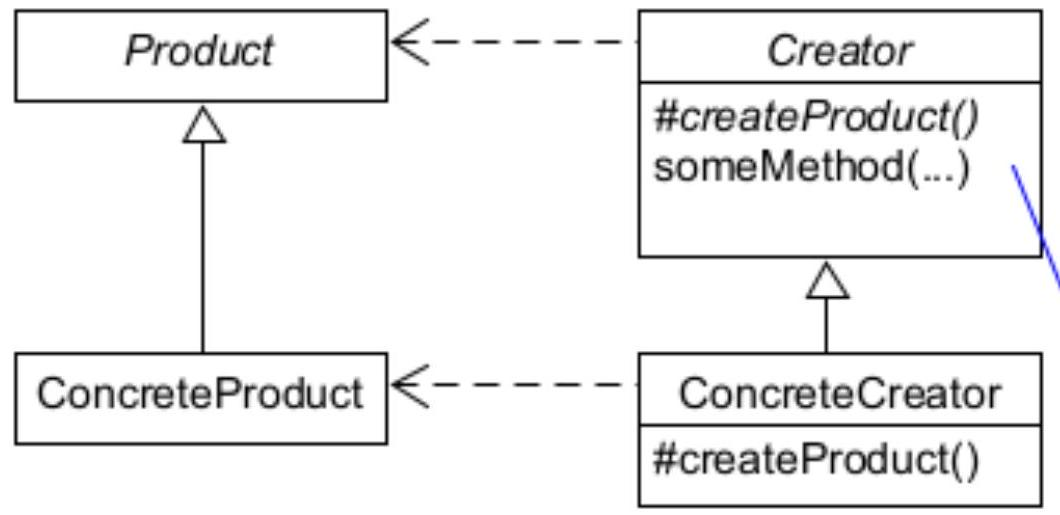
\includegraphics[width=0.6\linewidth]{images/2025_01_02_73d93f10fa91ab6123dcg-16}
\end{concept}

\begin{concept}{Abstract Factory}\\
\textbf{Problem:} Erzeugung verschiedener, zusammengehörender Objekte ohne Kenntnis konkreter Klassen\\
\textbf{Lösung:}
\begin{itemize}
    \item AbstractFactory-Interface definieren
    \item Pro Produkt eine create-Methode
    \item Konkrete Factories implementieren Interface
\end{itemize}
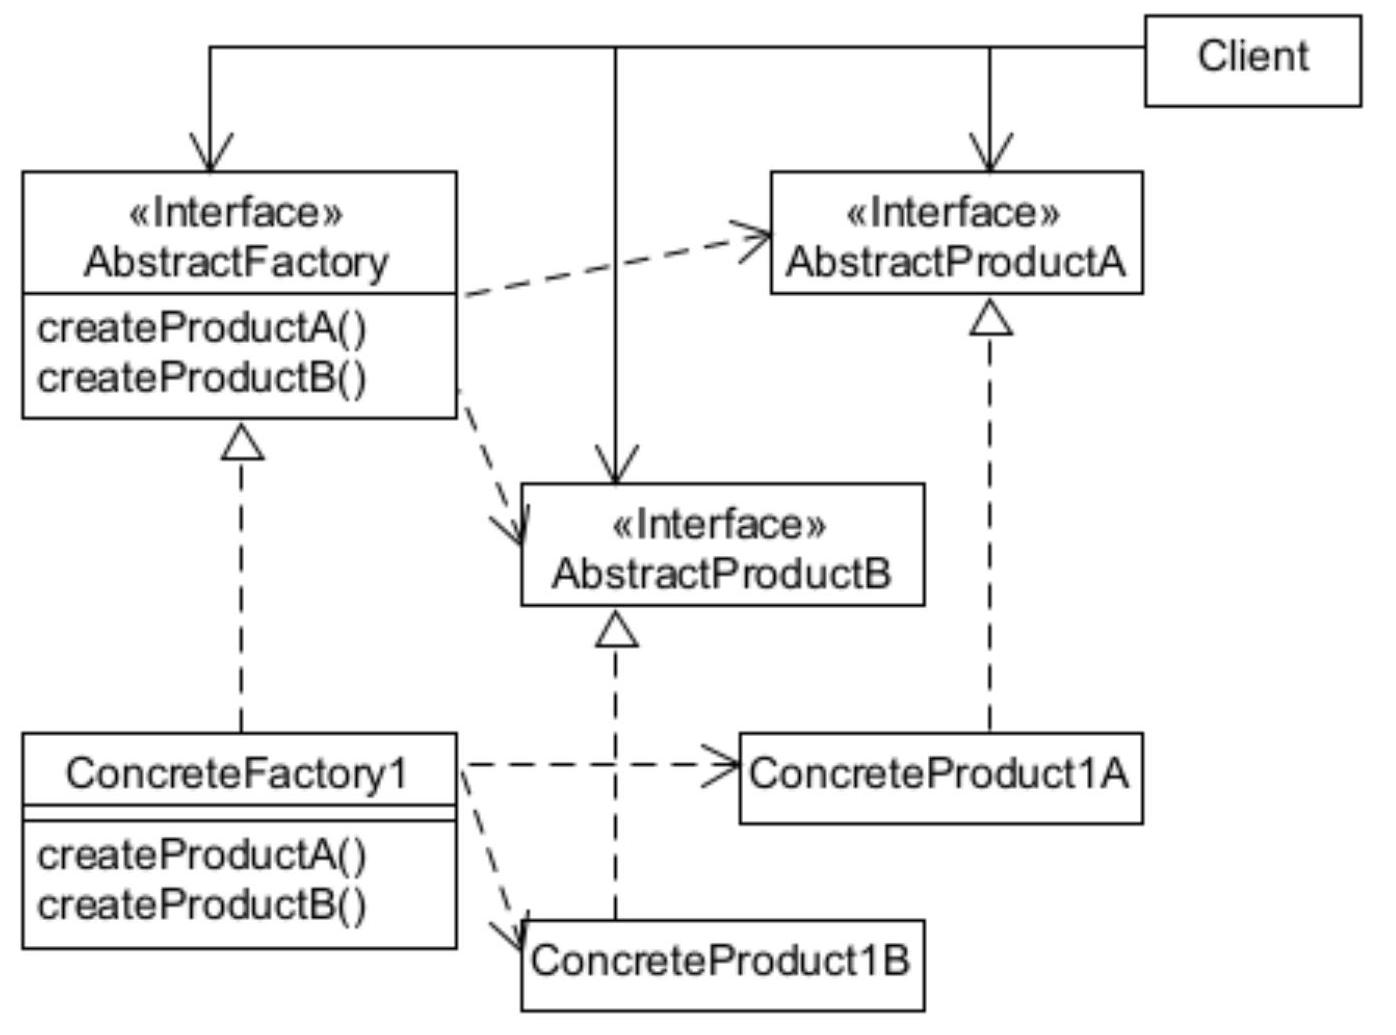
\includegraphics[width=0.8\linewidth]{images/2025_01_02_73d93f10fa91ab6123dcg-13}
\end{concept}


\begin{concept}{Command}\\
\textbf{Problem:} Aktionen für späteren Gebrauch speichern und verwalten\\
\textbf{Lösung:}
\begin{itemize}
    \item Command-Interface definieren
    \item Konkrete Commands implementieren
    \item Parameter für Ausführung speichern
    \item Optional: Undo-Funktionalität
\end{itemize}
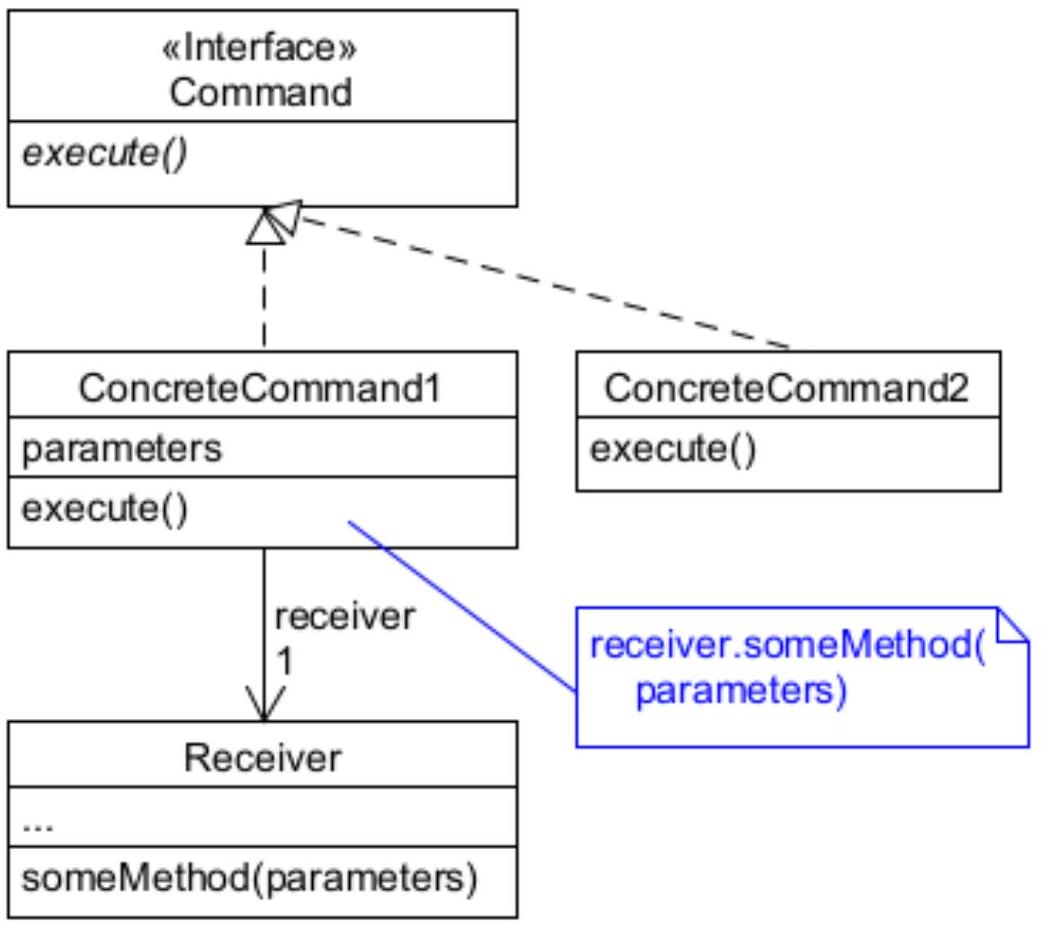
\includegraphics[width=0.7\linewidth]{images/2025_01_02_73d93f10fa91ab6123dcg-19}
\end{concept}


\begin{concept}{Template Method}\\
\textbf{Problem:} Algorithmus mit anpassbaren Teilschritten\\
\textbf{Lösung:}
\begin{itemize}
    \item Template Method in abstrakter Klasse
    \item Hook-Methoden für variable Teile
    \item Hollywood Principle: "Don't call us, we'll call you"
\end{itemize}
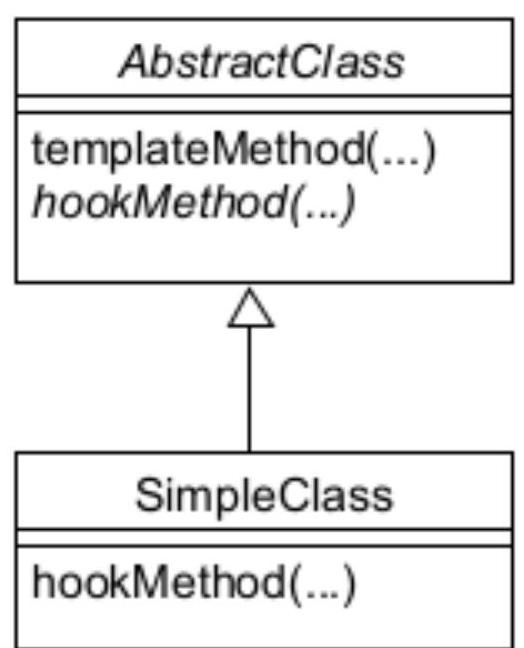
\includegraphics[width=0.3\linewidth]{images/2025_01_02_73d93f10fa91ab6123dcg-22}
\end{concept}

\begin{example2}{Framework Design Pattern Anwendung}\\
\textbf{Aufgabe:}
Implementieren Sie ein Plugin-System mit verschiedenen Design Patterns.

\textbf{Analyse der Pattern-Kombination:}
\begin{itemize}
    \item \textbf{Abstract Factory:}
    \begin{itemize}
        \item Plugin-Familie erzeugen
        \item Zusammengehörige Komponenten
        \item Austauschbare Implementierungen
    \end{itemize}
    
    \item \textbf{Template Method:}
    \begin{itemize}
        \item Plugin-Lifecycle definieren
        \item Standardablauf vorgeben
        \item Erweiterungspunkte bieten
    \end{itemize}
    
    \item \textbf{Command:}
    \begin{itemize}
        \item Plugin-Aktionen kapseln
        \item Asynchrone Ausführung
        \item Undo-Funktionalität
    \end{itemize}
\end{itemize}
\end{example2}


\subsection{Moderne Framework Mechanismen}

\begin{definition}{Annotation-basierte Konfiguration}\\
Moderne Frameworks nutzen Annotationen für:
\begin{itemize}
    \item Dependency Injection
    \item Konfiguration
    \item Interface-Implementation
    \item Funktionalitätserweiterung
\end{itemize}
\end{definition}

\begin{concept}{Annotations als Steuerungsmechanismus}\\
\textbf{Vorteile von Annotations:}
\begin{itemize}
    \item Keine harte Abhängigkeit zum Framework\\ (geringere Kopplung zur API)
    \item Annotation wird stillschweigend entfernt wenn nicht gefunden
    \item Geeignet für Domänenlogik ohne technische Abhängigkeiten
    \item Deklarativer Programmierstil
    \item Reduzierung von Boilerplate-Code
\end{itemize}

\textbf{Nachteil von Annotations:} Kann zu längeren Startzeiten führen
\end{concept}

\begin{theorem}{Auswertung von Annotations:}
\begin{itemize}
    \item \textbf{Startzeitpunkt:}
    \begin{itemize}
        \item Framework wird mit Anwendung gestartet
        \item Sucht Anwendungsklassen auf dem Klassenpfad
        \item Untersucht Annotationen
    \end{itemize}
    \item \textbf{Mögliche Framework-Aktionen:}
    \begin{itemize}
        \item Dependency Injection in Anwendungsobjekte
        \item Automatische Interface-Implementierung
        \item Funktionalität zu Klassen hinzufügen
    \end{itemize}
\end{itemize}
\end{theorem}

\begin{concept}{Aspekt-orientierte Programmierung in Frameworks}\\
\textbf{Querschnittliche Belange (Cross-Cutting Concerns):}
\begin{itemize}
    \item Logging
    \item Sicherheit
    \item Transaktionsmanagement
    \item Performance Monitoring
\end{itemize}

\textbf{Implementation mit Annotations:}
\begin{lstlisting}[language=Java, style=basesmol]
@Aspect
public class LoggingAspect {
    @Around("@annotation(Logged)")
    public Object logMethod(
            ProceedingJoinPoint joinPoint) 
            throws Throwable {
        
        String methodName = 
            joinPoint.getSignature().getName();
        Logger.info("Entering " + methodName);
        
        try {
            Object result = joinPoint.proceed();
            Logger.info("Exiting " + methodName);
            return result;
        } catch (Exception e) {
            Logger.error("Error in " + methodName, e);
            throw e;
        }
    }
}
// Usage in Framework Client Code
@Logged
public void businessMethod() {
    // Method implementation
}
\end{lstlisting}
\end{concept}



\begin{KR}{Java Mechanismen für Framework-Implementation}

    \begin{minipage}[t]{0.55\textwidth}
\textbf{1. Zeitpunkte für Code-Generierung}
\begin{itemize}
    \item \textbf{Compile-Zeit:}
    \begin{itemize}
        \item AnnotationProcessor
        \item Quellcode oder Bytecode generieren
    \end{itemize}
    \item \textbf{Laufzeit:}
    \begin{itemize}
        \item Beim Laden der Klassen
        \item Framework-Classloader
        \item Bytecode-Modifikation
    \end{itemize}
\end{itemize}
\end{minipage}
\begin{minipage}[t]{0.45\textwidth}
\textbf{2. Implementierungstechniken}
\begin{itemize}
    \item \textbf{Code Generation:}
    \begin{itemize}
        \item Quellcode hinzufügen
        \item Bytecode modifizieren
    \end{itemize}
    \item \textbf{Proxy Generation:}
    \begin{itemize}
        \item java.lang.reflect.Proxy
        \item Interface-Implementation
    \end{itemize}
\end{itemize}
\end{minipage}
\end{KR}

\begin{formula}{Framework Evaluation}

    \begin{minipage}[t]{0.5\textwidth}
\textbf{1. Qualitätskriterien}
\begin{itemize}
    \item \textbf{Usability:}
    \begin{itemize}
        \item Intuitive API
        \item Gute Dokumentation
        \item Beispiele/Templates
    \end{itemize}
    
    \item \textbf{Flexibilität:}
    \begin{itemize}
        \item Erweiterbarkeit
        \item Konfigurierbarkeit
        \item Modularität
    \end{itemize}
    
    \item \textbf{Wartbarkeit:}
    \begin{itemize}
        \item Klare Struktur
        \item Testbarkeit
        \item Versionierung
    \end{itemize}
\end{itemize}
\end{minipage}
\begin{minipage}[t]{0.5\textwidth}
\textbf{2. Risikobewertung}
\begin{itemize}
    \item \textbf{Technisch:}
    \begin{itemize}
        \item Kompatibilität
        \item Performance
        \item Skalierbarkeit
    \end{itemize}
    
    \item \textbf{Organisatorisch:}
    \begin{itemize}
        \item Learning Curve
        \item Support/Community
        \item Zukunftssicherheit
    \end{itemize}
\end{itemize}
\end{minipage}
\end{formula}

\begin{example2}{Prüfungsaufgabe: Framework Design Entscheidungen}\\
\textbf{Szenario:}
Sie sollen für eine Firma ein Framework zum Verarbeiten von Datenexporten entwickeln.
Die Firma arbeitet mit verschiedenen Datenformaten (CSV, Excel, XML) und möchte das 
Framework später einfach um weitere Formate erweitern können.

\textbf{Aufgabenstellung:}
\begin{enumerate}
    \item Identifizieren Sie die Variationspunkte
    \item Wählen Sie geeignete Design Patterns
    \item Skizzieren Sie die Framework-Architektur
\end{enumerate}

\textbf{Musterlösung:}
\begin{itemize}
    \item \textbf{Variationspunkte:}
    \begin{itemize}
        \item Format-Erkennung
        \item Datei-Parser
        \item Daten-Transformation
        \item Export-Ziele
    \end{itemize}
    
    \item \textbf{Design Patterns:}
    \begin{itemize}
        \item Abstract Factory für Parser-Erzeugung
        \item Strategy für unterschiedliche Parse-Algorithmen
        \item Template Method für generellen Export-Workflow
        \item Chain of Responsibility für Format-Erkennung
    \end{itemize}
    
    \item \textbf{Framework-Architektur:}
    \begin{itemize}
        \item Core API mit Interfaces
        \item Plugin-System für neue Formate
        \item Event-System für Export-Status
        \item Konfigurationsschicht
    \end{itemize}
\end{itemize}
\end{example2}

\columnbreak

\begin{example2}{Framework Design Pattern Kombination}\\
\textbf{Aufgabe:} 
Analysieren Sie die Kombination verschiedener Design Patterns in einem Framework.

\textbf{Muster-Framework:}
Event-Processing Framework mit folgenden Patterns:

\textbf{1. Template Method}
\begin{itemize}
    \item Definiert Workflow für Event-Verarbeitung
    \item Hook-Methoden für:
    \begin{itemize}
        \item Event-Validierung
        \item Event-Transformation
        \item Event-Persistierung
    \end{itemize}
\end{itemize}

\textbf{2. Chain of Responsibility}
\begin{itemize}
    \item Event-Handler-Kette
    \item Flexible Verarbeitungsreihenfolge
    \item Dynamische Handler-Registration
\end{itemize}

\textbf{3. Command}
\begin{itemize}
    \item Kapselung von Event-Handling-Logik
    \item Queuing von Events
    \item Undo/Redo Funktionalität
\end{itemize}

\textbf{4. Observer}
\begin{itemize}
    \item Benachrichtigung über Event-Status
    \item Lose Kopplung zwischen Komponenten
    \item Flexible Registration von Listeners
\end{itemize}

\textbf{Pattern-Interaktion:}
\begin{itemize}
    \item Template Method definiert Grundstruktur
    \item Chain of Responsibility organisiert Handler
    \item Command kapselt konkrete Aktionen
    \item Observer informiert über Ergebnisse
\end{itemize}
\end{example2}

\begin{example2}{Prüfungsaufgabe: Framework Testing}\\
\textbf{Szenario:}
Ein Framework soll gründlich getestet werden. Entwickeln Sie eine Teststrategie.

\textbf{Testebenen:}
\begin{itemize}
    \item \textbf{Unit Tests:}
    \begin{itemize}
        \item Einzelne Komponenten
        \item Mock-Objekte für Dependencies
        \item Edge Cases
    \end{itemize}
    
    \item \textbf{Integration Tests:}
    \begin{itemize}
        \item Zusammenspiel der Komponenten
        \item Plugin-Mechanismen
        \item Event-Handling
    \end{itemize}
    
    \item \textbf{System Tests:}
    \begin{itemize}
        \item End-to-End Szenarien
        \item Performance Tests 
        \item Load Tests
    \end{itemize}
\end{itemize}

\textbf{Besondere Aspekte:}
\begin{itemize}
    \item Extension Points testen
    \item Verschiedene Konfigurationen
    \item Backward Compatibility
    \item Error Handling
\end{itemize}
\end{example2}

\columnbreak

\begin{KR}{Framework-Extensions entwickeln}\\
\textbf{1. Extension Points identifizieren}
\begin{itemize}
    \item Core-Funktionalität analysieren
    \item Variationspunkte bestimmen
    \item Interface-Hierarchie planen
\end{itemize}

\textbf{2. Extension Mechanismen}
\begin{itemize}
    \item \textbf{Interface-basiert:}
    \begin{lstlisting}[language=Java, style=basesmol]
public interface Plugin {
    void initialize();
    void shutdown();
    String getName();
}
    \end{lstlisting}
    
    \item \textbf{Annotation-basiert:}
    \begin{lstlisting}[language=Java, style=basesmol]
@Extension
public class CustomPlugin {
    @Initialize
    public void setup() { ... }
    
    @Shutdown
    public void cleanup() { ... }
}
    \end{lstlisting}
\end{itemize}

\textbf{3. Discovery Mechanism}
\begin{lstlisting}[language=Java, style=basesmol]
public class ExtensionLoader {
    public List<Plugin> loadPlugins() {
        ServiceLoader<Plugin> loader = 
            ServiceLoader.load(Plugin.class);
        return StreamSupport
            .stream(loader.spliterator(), false)
            .collect(Collectors.toList());
    }
}
\end{lstlisting}
\end{KR}

\begin{example2}{Prüfungsaufgabe: Framework Evolution}\\
\textbf{Ausgangslage:}
Ein bestehendes Framework soll um neue Funktionalität erweitert werden, ohne bestehende 
Clients zu beeinträchtigen.

\textbf{Analyse der Optionen:}
\begin{itemize}
    \item \textbf{Annotation-basierte Erweiterung:}
    \begin{itemize}
        \item Vorteile:
        \begin{itemize}
            \item Keine Änderung bestehender Interfaces
            \item Optionale Funktionalität
            \item Deklarativer Ansatz
        \end{itemize}
        \item Nachteile:
        \begin{itemize}
            \item Komplexere Verarbeitung
            \item Mögliche Performance-Einbußen
            \item Schwieriger zu debuggen
        \end{itemize}
    \end{itemize}
    
    \item \textbf{Interface-basierte Erweiterung:}
    \begin{itemize}
        \item Vorteile:
        \begin{itemize}
            \item Klare Kontrakte
            \item Compile-time Checks
            \item Einfache Dokumentation
        \end{itemize}
        \item Nachteile:
        \begin{itemize}
            \item Änderungen an Interfaces nötig
            \item Adapter für alte Clients
            \item Höherer Implementierungsaufwand
        \end{itemize}
    \end{itemize}
\end{itemize}
\end{example2}

\columnbreak

\begin{KR}{Framework Integration}
\begin{enumerate}
    \item \textbf{Convention over Configuration}
    \begin{itemize}
        \item Namenskonventionen einhalten
        \item Standard-Verhalten nutzen
        \item Nur Ausnahmen konfigurieren
    \end{itemize}
    
    \item \textbf{Dependency Injection}
    \begin{itemize}
        \item Abhängigkeiten deklarieren
        \item Framework übernimmt Injection
        \item Constructor- oder Setter-Injection
    \end{itemize}
    
    \item \textbf{Interface-basierte Entwicklung}
    \begin{itemize}
        \item Interfaces definieren
        \item Framework generiert Implementation
        \item Methodennamen als Spezifikation
    \end{itemize}
\end{enumerate}
\end{KR}




\begin{example2}{Framework Integration Case Study}\\
\textbf{Szenario:}
Integration eines Logging-Frameworks in eine bestehende Anwendung

\textbf{Anforderungen:}
\begin{itemize}
    \item Minimale Änderungen am bestehenden Code
    \item Konfigurierbare Log-Level
    \item Verschiedene Log-Ausgaben (Konsole, File, DB)
    \item Performance-Monitoring
\end{itemize}

\textbf{Lösung mit Framework Patterns:}
\begin{lstlisting}[language=Java, style=basesmol]
// Logger Interface
public interface Logger {
    void debug(String message);
    void info(String message);
    void error(String message, Throwable t);
}
// Abstract Factory fuer Logger
public interface LoggerFactory {
    Logger getLogger(Class<?> clazz);
}
// Decorator fuer Performance Monitoring
public class PerformanceLogger implements Logger {
    private final Logger delegate;
    private final MetricsCollector metrics;
    
    @Override
    public void info(String message) {
        long start = System.nanoTime();
        try {
            delegate.info(message);
        } finally {
            long duration = System.nanoTime() - start;
            metrics.recordLogDuration(duration);
        }
    }
    // Other methods...
}
// Framework Configuration
@Configuration
public class LoggingConfig {
    @Bean
    public LoggerFactory loggerFactory(
            MetricsCollector metrics) {
        return clazz -> {
            Logger baseLogger = // create base logger
            return new PerformanceLogger(
                baseLogger, metrics);
        };
    }
}
\end{lstlisting}
\end{example2}

\columnbreak

\begin{example2}{Typische Prüfungsaufgabe: Framework Migration}\\
\textbf{Szenario:}
Ein bestehendes System soll von einem proprietären Framework auf ein Standard-Framework 
migriert werden.

\textbf{Aufgabenstellung:}
\begin{itemize}
    \item Analysieren Sie die Herausforderungen
    \item Entwickeln Sie eine Migrationsstrategie
    \item Bewerten Sie Risiken
\end{itemize}

\textbf{Lösungsansatz:}
\begin{itemize}
    \item \textbf{Analyse:}
    \begin{itemize}
        \item Framework-Abhängigkeiten identifizieren
        \item Geschäftskritische Funktionen isolieren
        \item Testabdeckung prüfen
    \end{itemize}
    
    \item \textbf{Strategie:}
    \begin{itemize}
        \item Adapter für Framework-Bridging
        \item Schrittweise Migration
        \item Parallelbetrieb ermöglichen
    \end{itemize}
    
    \item \textbf{Risikominimierung:}
    \begin{itemize}
        \item Automated Testing
        \item Feature Toggles
        \item Rollback-Möglichkeit
    \end{itemize}
\end{itemize}
\end{example2}









\subsubsection{complete examples}

\begin{example2}{Framework Design: Validation Framework}\\
\textbf{Anforderungen:}
Ein Framework für Validierung von Geschäftsobjekten soll entwickelt werden.

\textbf{Design:}
\begin{lstlisting}[language=Java, style=basesmol]
// Validation Annotations
@Target(ElementType.FIELD)
@Retention(RetentionPolicy.RUNTIME)
public @interface NotNull {
    String message() default "Value cannot be null";
}

@Target(ElementType.FIELD)
@Retention(RetentionPolicy.RUNTIME)
public @interface Length {
    int min() default 0;
    int max() default Integer.MAX_VALUE;
    String message() default "Length must be between {min} and {max}";
}

// Business Object
public class Customer {
    @NotNull
    private String id;
    
    @NotNull
    @Length(min = 2, max = 50)
    private String name;
    
    // getters and setters
}

// Validator Interface
public interface Validator<T> {
    ValidationResult validate(T object);
}

// Framework Implementation
public class ValidationFramework {
    public static <T> ValidationResult validate(T object) {
        Class<?> clazz = object.getClass();
        ValidationResult result = new ValidationResult();
        
        for (Field field : clazz.getDeclaredFields()) {
            validateField(object, field, result);
        }
        
        return result;
    }
}
\end{lstlisting}

\textbf{Verwendung:}
\begin{lstlisting}[language=Java, style=basesmol]
Customer customer = new Customer();
customer.setName("J"); // too short

ValidationResult result = 
    ValidationFramework.validate(customer);
if (!result.isValid()) {
    System.out.println(result.getErrors());
}
\end{lstlisting}
\end{example2}

\begin{example2}{Framework Design Pattern: Event System}\\
\textbf{Anforderung:}
Ein Framework soll Benutzern ermöglichen, auf verschiedene Events zu reagieren.

\textbf{Implementation:}
\begin{lstlisting}[language=Java, style=basesmol]
// Event Base Class
public abstract class Event {
    private final LocalDateTime timestamp;
    
    protected Event() {
        this.timestamp = LocalDateTime.now();
    }
    
    public LocalDateTime getTimestamp() {
        return timestamp;
    }
}

// Concrete Event
public class UserCreatedEvent extends Event {
    private final String userId;
    
    public UserCreatedEvent(String userId) {
        this.userId = userId;
    }
}

// Event Listener Interface
public interface EventListener<T extends Event> {
    void onEvent(T event);
}

// Event Bus
public class EventBus {
    private Map<Class<? extends Event>, 
               List<EventListener>> listeners = new HashMap<>();
    
    public <T extends Event> void register(
            Class<T> eventType, 
            EventListener<T> listener) {
        listeners.computeIfAbsent(eventType, 
            k -> new ArrayList<>()).add(listener);
    }
    
    public void publish(Event event) {
        List<EventListener> eventListeners = 
            listeners.get(event.getClass());
        if (eventListeners != null) {
            eventListeners.forEach(
                listener -> listener.onEvent(event));
        }
    }
}
\end{lstlisting}

\textbf{Framework Nutzung:}
\begin{lstlisting}[language=Java, style=basesmol]
// Framework Usage
EventBus eventBus = new EventBus();

// Register Listener
eventBus.register(UserCreatedEvent.class, 
    event -> System.out.println("User created: " 
        + event.getUserId()));

// Publish Event
eventBus.publish(new UserCreatedEvent("user123"));
\end{lstlisting}
\end{example2}
	\raggedcolumns
	\pagebreak
    \section{Framework Design}

\begin{concept}{Framework Grundlagen}\\
Ein Framework ist ein Programmiergerüst mit folgenden Eigenschaften:
\begin{itemize}
    \item Bietet wiederverwendbare Funktionalität
    \item Definiert Erweiterungs- und Anpassungspunkte
    \item Verwendet Design Patterns
    \item Enthält keinen applikationsspezifischen Code
    \item Gibt Rahmen für anwendungsspezifischen Code vor
    \item Klassen arbeiten eng zusammen (vs. reine Bibliothek)
\end{itemize}
\end{concept}

\begin{definition}{Framework Entwicklung}\\
Die Entwicklung eines Frameworks erfordert:
\begin{itemize}
    \item Höhere Zuverlässigkeit als normale Software
    \item Tiefergehende Analyse der Erweiterungspunkte
    \item Hoher Architektur- und Designaufwand
    \item Sorgfältige Planung der Schnittstellen
\end{itemize}
\end{definition}

\begin{remark}{Kritische Betrachtung}\\
Herausforderungen beim Framework-Einsatz:
\begin{itemize}
    \item Frameworks tendieren zu wachsender Funktionalität
    \item Gefahr von inkonsistentem Design
    \item Funktionale Überschneidungen möglich
    \item Hoher Einarbeitungsaufwand
    \item Schwierige "Scheidung" nach Integration
    \item Trade-off zwischen Abhängigkeit und Nutzen
\end{itemize}
\end{remark}

\subsection{Design Patterns in Frameworks}

\begin{concept}{Abstract Factory}\\
\textbf{Problem:} Erzeugung verschiedener, zusammengehörender Objekte ohne Kenntnis konkreter Klassen\\
\textbf{Lösung:}
\begin{itemize}
    \item AbstractFactory-Interface definieren
    \item Pro Produkt eine create-Methode
    \item Konkrete Factories implementieren Interface
\end{itemize}
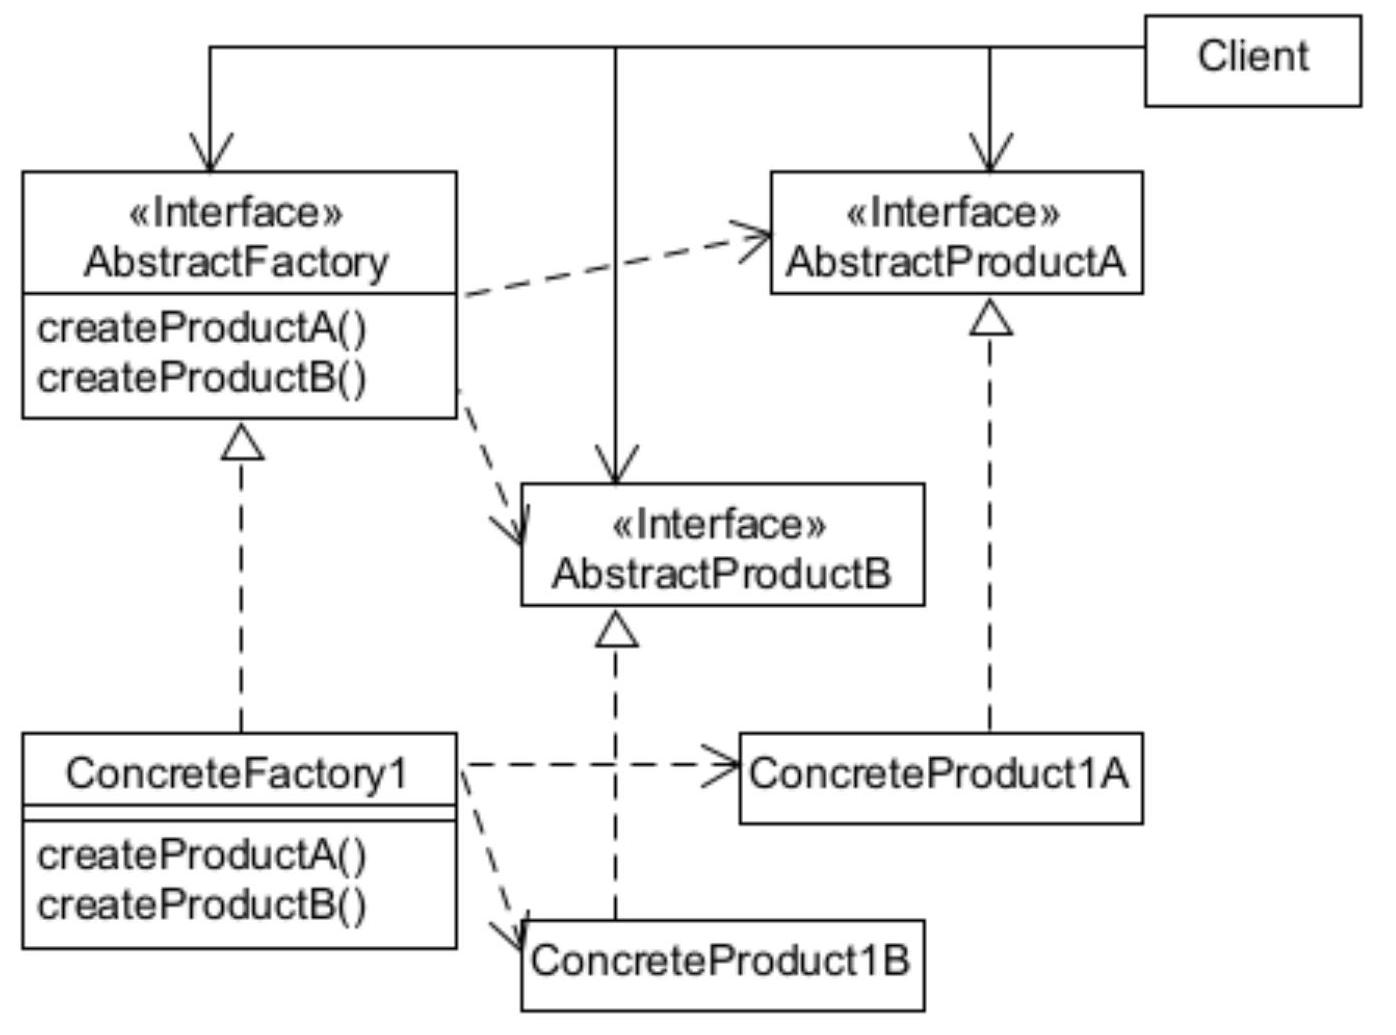
\includegraphics[width=0.8\linewidth]{images/2025_01_02_73d93f10fa91ab6123dcg-13}
\end{concept}

\begin{example}{Abstract Factory: POS Terminal}
\begin{lstlisting}[language=Java, style=base]
public interface IJavaPOSDevicesFactory {
    CashDrawer getNewCashDrawer();
    CoinDispenser getNewCoinDispenser();
    // weitere Methoden
}

public class IBMJavaPOSDevicesFactory 
        implements IJavaPOSDevicesFactory {
    public CashDrawer getNewCashDrawer() {
        return new com.ibm.pos.jpos.CashDrawer();
    }
    // weitere Implementierungen
}
\end{lstlisting}
\end{example}

\begin{concept}{Factory Method}\\
\textbf{Problem:} Flexible Objekterzeugung in wiederverwendbarer Klasse\\
\textbf{Lösung:}
\begin{itemize}
    \item Abstrakte Factory-Methode in Creator-Klasse
    \item Konkrete Subklassen überschreiben Methode
    \item Parallele Vererbungshierarchien
\end{itemize}
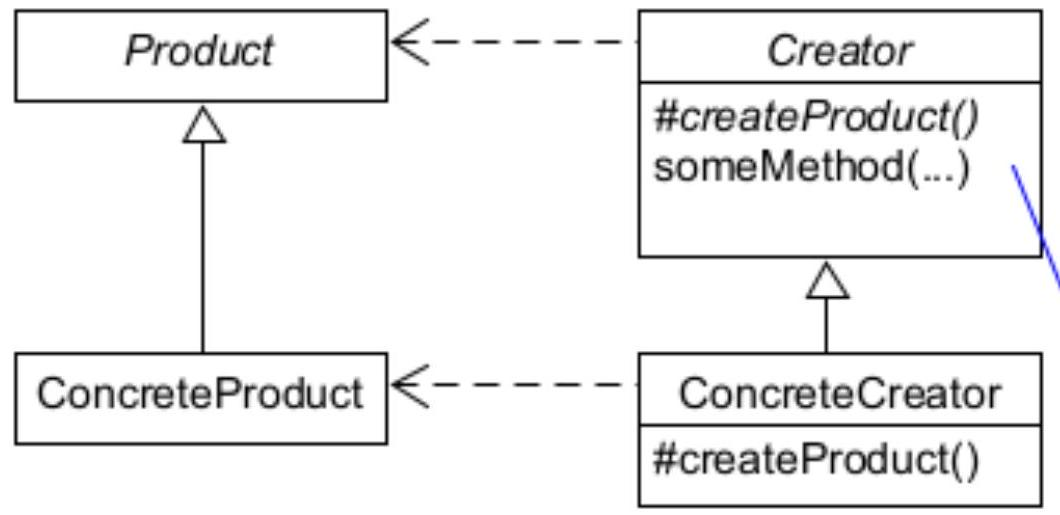
\includegraphics[width=0.8\linewidth]{images/2025_01_02_73d93f10fa91ab6123dcg-16}
\end{concept}

\begin{concept}{Command}\\
\textbf{Problem:} Aktionen für späteren Gebrauch speichern und verwalten\\
\textbf{Lösung:}
\begin{itemize}
    \item Command-Interface definieren
    \item Konkrete Commands implementieren
    \item Parameter für Ausführung speichern
    \item Optional: Undo-Funktionalität
\end{itemize}
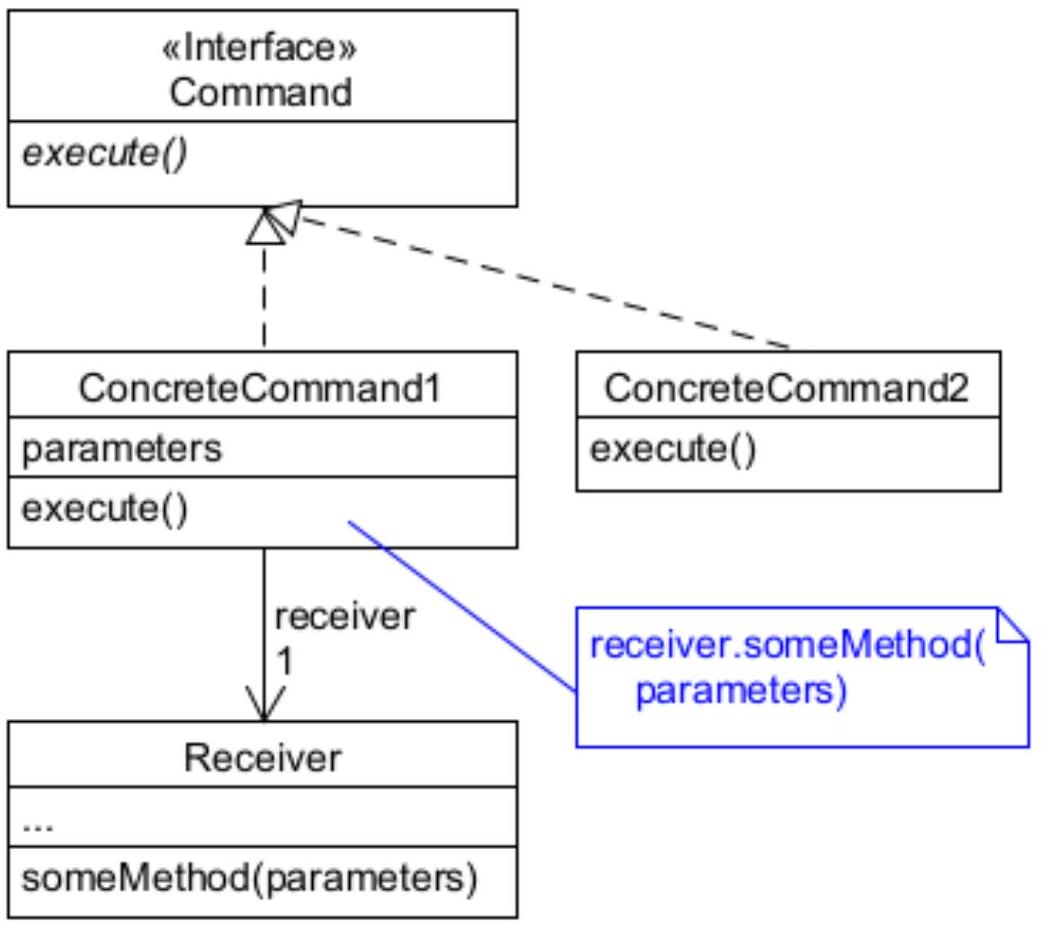
\includegraphics[width=0.8\linewidth]{images/2025_01_02_73d93f10fa91ab6123dcg-19}
\end{concept}

\begin{example}{Command: Persistenz}
\begin{lstlisting}[language=Java, style=base]
public interface ICommand {
    void execute();
    void undo();
}

public class DBUpdateCommand implements ICommand {
    private PersistentObject object;
    
    public void execute() {
        // Update in Datenbank
    }
    
    public void undo() {
        // Aenderung rueckgaengig machen
    }
}
\end{lstlisting}
\end{example}

\begin{concept}{Template Method}\\
\textbf{Problem:} Algorithmus mit anpassbaren Teilschritten\\
\textbf{Lösung:}
\begin{itemize}
    \item Template Method in abstrakter Klasse
    \item Hook-Methoden für variable Teile
    \item Hollywood Principle: "Don't call us, we'll call you"
\end{itemize}
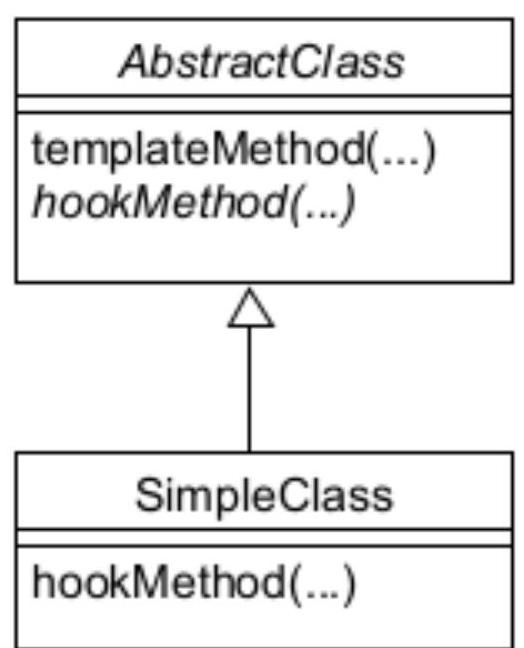
\includegraphics[width=0.8\linewidth]{images/2025_01_02_73d93f10fa91ab6123dcg-22}
\end{concept}

\begin{example}{Template Method: GUI Framework}
\begin{lstlisting}[language=Java, style=base]
public abstract class GUIComponent {
    // Template Method
    public final void update() {
        clearBackground();
        repaint(); // Hook Method
    }
    
    protected abstract void repaint();
}

public class MyButton extends GUIComponent {
    protected void repaint() {
        // Button-spezifische Implementation
    }
}
\end{lstlisting}
\end{example}

\subsection{Moderne Framework Patterns}

\begin{concept}{Annotation-basierte Konfiguration}\\
Moderne Frameworks nutzen Annotationen für:
\begin{itemize}
    \item Dependency Injection
    \item Konfiguration
    \item Interface-Implementation
    \item Funktionalitätserweiterung
\end{itemize}
\end{concept}

\begin{KR}{Framework Integration}
\begin{enumerate}
    \item \textbf{Convention over Configuration}
    \begin{itemize}
        \item Namenskonventionen einhalten
        \item Standard-Verhalten nutzen
        \item Nur Ausnahmen konfigurieren
    \end{itemize}
    
    \item \textbf{Dependency Injection}
    \begin{itemize}
        \item Abhängigkeiten deklarieren
        \item Framework übernimmt Injection
        \item Constructor- oder Setter-Injection
    \end{itemize}
    
    \item \textbf{Interface-basierte Entwicklung}
    \begin{itemize}
        \item Interfaces definieren
        \item Framework generiert Implementation
        \item Methodennamen als Spezifikation
    \end{itemize}
\end{enumerate}
\end{KR}

\begin{example}{Spring Data Repository}
\begin{lstlisting}[language=Java, style=base]
@Repository
public interface UserRepository 
        extends JpaRepository<User, Long> {
    // Methode wird automatisch implementiert
    List<User> findByLastNameOrderByFirstNameAsc(
        String lastName);
    
    // SQL-Query via Annotation
    @Query("SELECT u FROM User u WHERE u.active = true")
    List<User> findActiveUsers();
}
\end{lstlisting}
\end{example}

\begin{remark}
Annotation-basierte Frameworks bieten:
\begin{itemize}
    \item Geringere Kopplung zur Framework-API
    \item Deklarativen Programmierstil
    \item Reduzierte Boilerplate-Code
    \item Kann aber zu längeren Startzeiten führen
\end{itemize}
\end{remark}
	\raggedcolumns
	
\end{multicols}
\end{document}